%********************************************%
%*       Generated from PreTeXt source      *%
%*       on 2024-12-10T16:07:50-05:00       *%
%*   A recent stable commit (2022-07-01):   *%
%* 6c761d3dba23af92cba35001c852aac04ae99a5f *%
%*                                          *%
%*         https://pretextbook.org          *%
%*                                          *%
%********************************************%
\documentclass[twoside, 14pt]{extarticle}
%% Custom Preamble Entries, early (use latex.preamble.early)
%% Always open on odd page
%%   The following adjusts cleardoublepage to remove twosided
%%   check so that we open on odd pages even in one-sided mode
%%   by adding an extra blank page on the preceding even page.
\makeatletter%
\def\cleardoublepage{%
\clearpage\ifodd\c@page\else\thispagestyle{empty}\hbox{}\newpage\if@twocolumn\hbox{}\newpage\fi\fi%
}
\makeatother%
%% Default LaTeX packages
%%   1.  always employed (or nearly so) for some purpose, or
%%   2.  a stylewriter may assume their presence
\usepackage{geometry}
%% Some aspects of the preamble are conditional,
%% the LaTeX engine is one such determinant
\usepackage{ifthen}
%% etoolbox has a variety of modern conveniences
\usepackage{etoolbox}
\usepackage{ifxetex,ifluatex}
%% Raster graphics inclusion
\usepackage{graphicx}
%% Color support, xcolor package
%% Always loaded, for: add/delete text, author tools
%% Here, since tcolorbox loads tikz, and tikz loads xcolor
\PassOptionsToPackage{usenames,dvipsnames,svgnames,table}{xcolor}
\usepackage{xcolor}
%% begin: defined colors, via xcolor package, for styling
%% end: defined colors, via xcolor package, for styling
%% Colored boxes, and much more, though mostly styling
%% skins library provides "enhanced" skin, employing tikzpicture
%% boxes may be configured as "breakable" or "unbreakable"
%% "raster" controls grids of boxes, aka side-by-side
\usepackage{comment}
\usepackage{tcolorbox}
\tcbuselibrary{skins}
\tcbuselibrary{breakable}
\tcbuselibrary{raster}
%% We load some "stock" tcolorbox styles that we use a lot
%% Placement here is provisional, there will be some color work also
%% First, black on white, no border, transparent, but no assumption about titles
\tcbset{ bwminimalstyle/.style={enhanced, frame empty, extras broken={
          frame empty}, fonttitle=\bfseries, colback=white, colbacktitle=black!20, coltitle=black, opacityfill=1.0, } }
%% Second, bold title, run-in to text/paragraph/heading
%% Space afterwards will be controlled by environment,
%% independent of constructions of the tcb title
%% Places \blocktitlefont onto many block titles
\tcbset{ runintitlestyle/.style={fonttitle=\blocktitlefont\upshape\bfseries, attach title to upper} }
%% Spacing prior to each exercise, anywhere
\tcbset{ exercisespacingstyle/.style={before skip={1.5ex plus 0.5ex}} }
%% Spacing prior to each block
\tcbset{ blockspacingstyle/.style={before skip={2.0ex plus 0.5ex}} }
%% xparse allows the construction of more robust commands,
%% this is a necessity for isolating styling and behavior
%% The tcolorbox library of the same name loads the base library
\tcbuselibrary{xparse}
%% The tcolorbox library loads TikZ, its calc package is generally useful,
%% and is necessary for some smaller documents that use partial tcolor boxes
%% See:  https://github.com/PreTeXtBook/pretext/issues/1624
\usetikzlibrary{calc}
%% We use some more exotic tcolorbox keys to restore indentation to parboxes
\tcbuselibrary{hooks}
%% Save default paragraph indentation for use later, when adjusting parboxes
\newlength{\normalparindent}
\AtBeginDocument{\setlength{\normalparindent}{\parindent}}
%% Hyperref should be here, but likes to be loaded late
%%
%% Inline math delimiters, \(, \), need to be robust
%% 2016-01-31:  latexrelease.sty  supersedes  fixltx2e.sty
%% If  latexrelease.sty  exists, bugfix is in kernel
%% If not, bugfix is in  fixltx2e.sty
%% See:  https://tug.org/TUGboat/tb36-3/tb114ltnews22.pdf
%% and read "Fewer fragile commands" in distribution's  latexchanges.pdf
\IfFileExists{latexrelease.sty}{}{\usepackage{fixltx2e}}
%% shorter subnumbers in some side-by-side require manipulations
\usepackage{xstring}
%% Footnote counters and part/chapter counters are manipulated
%% April 2018:  chngcntr  commands now integrated into the kernel,
%% but circa 2018/2019 the package would still try to redefine them,
%% so we need to do the work of loading conditionally for old kernels.
%% From version 1.1a,  chngcntr  should detect defintions made by LaTeX kernel.
\ifdefined\counterwithin
\else
    \usepackage{chngcntr}
\fi
%% Text height identically 9 inches, text width varies on point size
%% See Bringhurst 2.1.1 on measure for recommendations
%% 75 characters per line (count spaces, punctuation) is target
%% which is the upper limit of Bringhurst's recommendations
\geometry{letterpaper, inner=1in, outer=0.7in, top=0.4in, bottom=0.7in}
%% Custom Page Layout Adjustments (use publisher page-geometry entry)
%% This LaTeX file may be compiled with pdflatex, xelatex, or lualatex executables
%% LuaTeX is not explicitly supported, but we do accept additions from knowledgeable users
%% The conditional below provides  pdflatex  specific configuration last
%% begin: engine-specific capabilities
\ifthenelse{\boolean{xetex} \or \boolean{luatex}}{%
%% begin: xelatex and lualatex-specific default configuration
\ifxetex\usepackage{xltxtra}\fi
%% realscripts is the only part of xltxtra relevant to lualatex 
\ifluatex\usepackage{realscripts}\fi
%% end:   xelatex and lualatex-specific default configuration
}{
%% begin: pdflatex-specific default configuration
%% We assume a PreTeXt XML source file may have Unicode characters
%% and so we ask LaTeX to parse a UTF-8 encoded file
%% This may work well for accented characters in Western language,
%% but not with Greek, Asian languages, etc.
%% When this is not good enough, switch to the  xelatex  engine
%% where Unicode is better supported (encouraged, even)
\usepackage[utf8]{inputenc}
%% end: pdflatex-specific default configuration
}
%% end:   engine-specific capabilities
%%
%% Fonts.  Conditional on LaTex engine employed.
%% Default Text Font: The Latin Modern fonts are
%% "enhanced versions of the [original TeX] Computer Modern fonts."
%% We use them as the default text font for PreTeXt output.
%% Default Monospace font: Inconsolata (aka zi4)
%% Sponsored by TUG: http://levien.com/type/myfonts/inconsolata.html
%% Loaded for documents with intentional objects requiring monospace
%% See package documentation for excellent instructions
%% fontspec will work universally if we use filename to locate OTF files
%% Loads the "upquote" package as needed, so we don't have to
%% Upright quotes might come from the  textcomp  package, which we also use
%% We employ the shapely \ell to match Google Font version
%% pdflatex: "varl" package option produces shapely \ell
%% pdflatex: "var0" package option produces plain zero (not used)
%% pdflatex: "varqu" package option produces best upright quotes
%% xelatex,lualatex: add OTF StylisticSet 1 for shapely \ell
%% xelatex,lualatex: add OTF StylisticSet 2 for plain zero (not used)
%% xelatex,lualatex: add OTF StylisticSet 3 for upright quotes
%%
%% Fancy Verbatim for consoles, preformatted, code display, literate programming
\usepackage{fancyvrb}
%% Pre-formatted text, a peer of paragraphs
\DefineVerbatimEnvironment{preformatted}{Verbatim}{}
%% Automatic Font Control
%% Portions of a document, are, or may, be affected by defined commands
%% These are perhaps more flexible when using  xelatex  rather than  pdflatex
%% The following definitions are meant to be re-defined in a style, using \renewcommand
%% They are scoped when employed (in a TeX group), and so should not be defined with an argument
\newcommand{\divisionfont}{\relax}
\newcommand{\blocktitlefont}{\relax}
\newcommand{\contentsfont}{\relax}
\newcommand{\pagefont}{\relax}
\newcommand{\tabularfont}{\relax}
\newcommand{\xreffont}{\relax}
\newcommand{\titlepagefont}{\relax}
%%
\ifthenelse{\boolean{xetex} \or \boolean{luatex}}{%
%% begin: font setup and configuration for use with xelatex
%% Generally, xelatex is necessary for non-Western fonts
%% fontspec package provides extensive control of system fonts,
%% meaning *.otf (OpenType), and apparently *.ttf (TrueType)
%% that live *outside* your TeX/MF tree, and are controlled by your *system*
%% (it is possible that a TeX distribution will place fonts in a system location)
%%
%% The fontspec package is the best vehicle for using different fonts in  xelatex
%% So we load it always, no matter what a publisher or style might want
%%
\usepackage{fontspec}
%%
%% begin: xelatex main font ("font-xelatex-main" template)
%% Latin Modern Roman is the default font for xelatex and so is loaded with a TU encoding
%% *in the format* so we can't touch it, only perhaps adjust it later
%% in one of two ways (then known by NFSS names such as "lmr")
%% (1) via NFSS with font family names such as "lmr" and "lmss"
%% (2) via fontspec with commands like \setmainfont{Latin Modern Roman}
%% The latter requires the font to be known at the system-level by its font name,
%% but will give access to OTF font features through optional arguments
%% https://tex.stackexchange.com/questions/470008/
%% where-and-how-does-fontspec-sty-specify-the-default-font-latin-modern-roman
%% http://tex.stackexchange.com/questions/115321
%% /how-to-optimize-latin-modern-font-with-xelatex
%%
%% end:   xelatex main font ("font-xelatex-main" template)
%% begin: xelatex mono font ("font-xelatex-mono" template)
%% (conditional on non-trivial uses being present in source)
\IfFontExistsTF{Inconsolatazi4-Regular.otf}{}{\GenericError{}{The font "Inconsolatazi4-Regular.otf" requested by PreTeXt output is not available.  Either a file cannot be located in default locations via a filename, or a font is not known by its name as part of your system.}{Consult the PreTeXt Guide for help with LaTeX fonts.}{}}
\IfFontExistsTF{Inconsolatazi4-Bold.otf}{}{\GenericError{}{The font "Inconsolatazi4-Bold.otf" requested by PreTeXt output is not available.  Either a file cannot be located in default locations via a filename, or a font is not known by its name as part of your system.}{Consult the PreTeXt Guide for help with LaTeX fonts.}{}}
\usepackage{zi4}
\setmonofont[BoldFont=Inconsolatazi4-Bold.otf,StylisticSet={1,3}]{Inconsolatazi4-Regular.otf}
%% end:   xelatex mono font ("font-xelatex-mono" template)
%% begin: xelatex font adjustments ("font-xelatex-style" template)
%% end:   xelatex font adjustments ("font-xelatex-style" template)
%%
%% Extensive support for other languages
\usepackage{polyglossia}
%% Set main/default language based on pretext/@xml:lang value
%% document language code is "es-ES", Spanish
\setmainlanguage{spanish}
%% Enable secondary languages based on discovery of @xml:lang values
%% Enable fonts/scripts based on discovery of @xml:lang values
%% Western languages should be ably covered by Latin Modern Roman
%% end:   font setup and configuration for use with xelatex
}{%
%% begin: font setup and configuration for use with pdflatex
%% begin: pdflatex main font ("font-pdflatex-main" template)
\usepackage{lmodern}
\usepackage[T1]{fontenc}
%% end:   pdflatex main font ("font-pdflatex-main" template)
%% begin: pdflatex mono font ("font-pdflatex-mono" template)
%% (conditional on non-trivial uses being present in source)
\usepackage[varqu,varl]{inconsolata}
%% end:   pdflatex mono font ("font-pdflatex-mono" template)
%% begin: pdflatex font adjustments ("font-pdflatex-style" template)
%% end:   pdflatex font adjustments ("font-pdflatex-style" template)
%% end:   font setup and configuration for use with pdflatex
}
%% Micromanage spacing, etc.  The named "microtype-options"
%% template may be employed to fine-tune package behavior
\usepackage{microtype}
%% Symbols, align environment, commutative diagrams, bracket-matrix
\usepackage{amsmath}
\usepackage{amscd}
\usepackage{amssymb}
%% allow page breaks within display mathematics anywhere
%% level 4 is maximally permissive
%% this is exactly the opposite of AMSmath package philosophy
%% there are per-display, and per-equation options to control this
%% split, aligned, gathered, and alignedat are not affected
\allowdisplaybreaks[4]
%% allow more columns to a matrix
%% can make this even bigger by overriding with  latex.preamble.late  processing option
\setcounter{MaxMatrixCols}{30}
%%
%%
%% Division Titles, and Page Headers/Footers
%% titlesec package, loading "titleps" package cooperatively
%% See code comments about the necessity and purpose of "explicit" option.
%% The "newparttoc" option causes a consistent entry for parts in the ToC 
%% file, but it is only effective if there is a \titleformat for \part.
%% "pagestyles" loads the  titleps  package cooperatively.
\usepackage[explicit, newparttoc, pagestyles]{titlesec}
%% The companion titletoc package for the ToC.
\usepackage{titletoc}
%% begin: customizations of page styles via the modal "titleps-style" template
%% Designed to use commands from the LaTeX "titleps" package
\pagestyle{plain}
%% end: customizations of page styles via the modal "titleps-style" template
%%
%% Create globally-available macros to be provided for style writers
%% These are redefined for each occurence of each division
%
% Number subsections ignoring sections
\renewcommand{\thesubsection}{\arabic{subsection}}
\makeatletter
\@removefromreset{subsection}{section}
\makeatother
%
%
\newcommand{\divisionnameptx}{\relax}%
\newcommand{\titleptx}{\relax}%
\newcommand{\subtitleptx}{\relax}%
\newcommand{\shortitleptx}{\relax}%
\newcommand{\authorsptx}{\relax}%
\newcommand{\epigraphptx}{\relax}%
\newcommand{\laLeccion}{\relax}
%% Create environments for possible occurences of each division
%% Environment for a PTX "section" at the level of a LaTeX "section"
\NewDocumentEnvironment{sectionptx}{mmmmmmm}
{%
\renewcommand{\divisionnameptx}{#1}%
\renewcommand{\titleptx}{#2}%
\renewcommand{\subtitleptx}{#3}%
\renewcommand{\shortitleptx}{#4}%
\renewcommand{\authorsptx}{#5}%
\renewcommand{\epigraphptx}{#6}%
% \section{}%[{#4}]{#2}%
% \label{#7}%
% \clearpage
}{}%
%% Environment for a PTX "subsection" at the level of a LaTeX "subsection"
\NewDocumentEnvironment{subsectionptx}{mmmmmmm}
{%
\renewcommand{\divisionnameptx}{#1}%
\renewcommand{\titleptx}{#2}%
\renewcommand{\subtitleptx}{#3}%
\renewcommand{\shortitleptx}{#4}%
\renewcommand{\authorsptx}{#5}%
\renewcommand{\epigraphptx}{#6}%
\renewcommand{\laLeccion}{#4}%
% \vspace{-1.5cm}
% \subsection{}%[{#4}]{#2}%
\label{#7}%
}{}%
%% Environment for a PTX "reading-questions" at the level of a LaTeX "subsubsection"
\NewDocumentEnvironment{reading-questions-subsubsection}{mmmmmmm}
{%
\renewcommand{\divisionnameptx}{#1}%
\renewcommand{\titleptx}{#2}%
\renewcommand{\subtitleptx}{#3}%
\renewcommand{\shortitleptx}{#4}%
\renewcommand{\authorsptx}{#5}%
\renewcommand{\epigraphptx}{#6}%
% \clearpage
% \vspace{-0.4cm}
% \subsubsection[{#4}]{\laLeccion~-~#2}%
% \vspace{-0.4cm}
% \label{#7}%
}{}%
%% Environment for a PTX "reading-questions" at the level of a LaTeX "subsubsection"
\NewDocumentEnvironment{reading-questions-subsubsection-numberless}{mmmmmmm}
{%
\renewcommand{\divisionnameptx}{#1}%
\renewcommand{\titleptx}{#2}%
\renewcommand{\subtitleptx}{#3}%
\renewcommand{\shortitleptx}{#4}%
\renewcommand{\authorsptx}{#5}%
\renewcommand{\epigraphptx}{#6}%
% \clearpage
% \vspace{-1.2cm}
% \subsubsection*{\laLeccion~-~#2}%
% \vspace{-0.4cm}
% \addcontentsline{toc}{subsubsection}{#4}
% \label{#7}%
}{}%
%% Environment for a PTX "subsubsection" at the level of a LaTeX "subsubsection"
\NewDocumentEnvironment{subsubsectionptx}{mmmmmmm}
{%
\renewcommand{\divisionnameptx}{#1}%
\renewcommand{\titleptx}{#2}%
\renewcommand{\subtitleptx}{#3}%
\renewcommand{\shortitleptx}{#4}%
\renewcommand{\authorsptx}{#5}%
\renewcommand{\epigraphptx}{#6}%
% \clearpage
\vspace{-0.7cm}
\subsubsection[{#4}]{\laLeccion~-~#2}%
\vspace{-0.7cm}
\label{#7}%
}{}%
%% Environment for a PTX "exercises" at the level of a LaTeX "subsection"
\NewDocumentEnvironment{exercises-subsection}{mmmmmmm}
{%
\renewcommand{\divisionnameptx}{#1}%
\renewcommand{\titleptx}{#2}%
\renewcommand{\subtitleptx}{#3}%
\renewcommand{\shortitleptx}{#4}%
\renewcommand{\authorsptx}{#5}%
\renewcommand{\epigraphptx}{#6}%
% \clearpage
% \subsection*{#2}%
% \label{#7}%
}{}%
%% Environment for a PTX "exercises" at the level of a LaTeX "subsection"
\NewDocumentEnvironment{exercises-subsection-numberless}{mmmmmmm}
{%
\renewcommand{\divisionnameptx}{#1}%
\renewcommand{\titleptx}{#2}%
\renewcommand{\subtitleptx}{#3}%
\renewcommand{\shortitleptx}{#4}%
\renewcommand{\authorsptx}{#5}%
\renewcommand{\epigraphptx}{#6}%
% \subsection*{#2}%
% \subsection[{#4}]{\laLeccion - #2}
% \addcontentsline{toc}{subsection}{\laLeccion - #4}
% \label{#7}%
}{}%
%% Environment for a PTX "references" at the level of a LaTeX "subsection"
\NewDocumentEnvironment{references-subsection}{mmmmmmm}
{%
\renewcommand{\divisionnameptx}{#1}%
\renewcommand{\titleptx}{#2}%
\renewcommand{\subtitleptx}{#3}%
\renewcommand{\shortitleptx}{#4}%
\renewcommand{\authorsptx}{#5}%
\renewcommand{\epigraphptx}{#6}%
\subsection[{#4}]{\laLeccion - #2}%
\label{#7}%
}{}%
%% Environment for a PTX "references" at the level of a LaTeX "subsection"
\NewDocumentEnvironment{references-subsection-numberless}{mmmmmmm}
{%
\renewcommand{\divisionnameptx}{#1}%
\renewcommand{\titleptx}{#2}%
\renewcommand{\subtitleptx}{#3}%
\renewcommand{\shortitleptx}{#4}%
\renewcommand{\authorsptx}{#5}%
\renewcommand{\epigraphptx}{#6}%
\subsection*{#2}%
\addcontentsline{toc}{subsection}{\laLeccion - #4}
\label{#7}%
}{}%
%% Environment for a PTX "references" at the level of a LaTeX "section"
\NewDocumentEnvironment{references-section}{mmmmmmm}
{%
\renewcommand{\divisionnameptx}{#1}%
\renewcommand{\titleptx}{#2}%
\renewcommand{\subtitleptx}{#3}%
\renewcommand{\shortitleptx}{#4}%
\renewcommand{\authorsptx}{#5}%
\renewcommand{\epigraphptx}{#6}%
\section[{#4}]{#2}%
\label{#7}%
}{}%
%% Environment for a PTX "references" at the level of a LaTeX "section"
\NewDocumentEnvironment{references-section-numberless}{mmmmmmm}
{%
\renewcommand{\divisionnameptx}{#1}%
\renewcommand{\titleptx}{#2}%
\renewcommand{\subtitleptx}{#3}%
\renewcommand{\shortitleptx}{#4}%
\renewcommand{\authorsptx}{#5}%
\renewcommand{\epigraphptx}{#6}%
\section*{#2}%
\addcontentsline{toc}{section}{#4}
\label{#7}%
}{}%
%%
%% Styles for six traditional LaTeX divisions
\titleformat{\part}[display]
{\divisionfont\Huge\bfseries\centering}{\divisionnameptx\space\thepart}{30pt}{\Huge#1}
[{\Large\centering\authorsptx}]
\titleformat{\chapter}[display]
{\divisionfont\huge\bfseries}{\divisionnameptx\space\thechapter}{20pt}{\Huge#1}
[{\Large\authorsptx}]
\titleformat{name=\chapter,numberless}[display]
{\divisionfont\huge\bfseries}{}{0pt}{#1}
[{\Large\authorsptx}]
\titlespacing*{\chapter}{0pt}{50pt}{40pt}
\titleformat{\section}[hang]
{\divisionfont\Large\bfseries}{}{1ex}{#1}
[{\large\authorsptx}]
\titleformat{name=\section,numberless}[block]
{\divisionfont\Large\bfseries}{}{0pt}{#1}
[{\large\authorsptx}]
\titlespacing*{\section}{0pt}{3.5ex plus 1ex minus .2ex}{2.3ex plus .2ex}
\titleformat{\subsection}[hang]
{\divisionfont\large\bfseries}{}{1ex}{#1}
[{\normalsize\authorsptx}]
\titleformat{name=\subsection,numberless}[block]
{\divisionfont\large\bfseries}{}{0pt}{#1}
[{\normalsize\authorsptx}]
\titlespacing*{\subsection}{0pt}{3.25ex plus 1ex minus .2ex}{1.5ex plus .2ex}
\titleformat{\subsubsection}[hang]
{\divisionfont\normalsize\bfseries}{\thesubsubsection}{1em}{#1}
[{\small\authorsptx}]
\titleformat{name=\subsubsection,numberless}[block]
{\divisionfont\normalsize\bfseries}{}{0pt}{#1}
[{\normalsize\authorsptx}]
\titlespacing*{\subsubsection}{0pt}{3.25ex plus 1ex minus .2ex}{1.5ex plus .2ex}
\titleformat{\paragraph}[hang]
{\divisionfont\normalsize\bfseries}{\theparagraph}{1em}{#1}
[{\small\authorsptx}]
\titleformat{name=\paragraph,numberless}[block]
{\divisionfont\normalsize\bfseries}{}{0pt}{#1}
[{\normalsize\authorsptx}]
\titlespacing*{\paragraph}{0pt}{3.25ex plus 1ex minus .2ex}{1.5em}
%%
%% Styles for five traditional LaTeX divisions
\titlecontents{part}%
[0pt]{\contentsmargin{0em}\addvspace{1pc}\contentsfont\bfseries}%
{\Large\thecontentslabel\enspace}{\Large}%
{}%
[\addvspace{.5pc}]%
\titlecontents{chapter}%
[0pt]{\contentsmargin{0em}\addvspace{1pc}\contentsfont\bfseries}%
{\large\thecontentslabel\enspace}{\large}%
{\hfill\bfseries\thecontentspage}%
[\addvspace{.5pc}]%
\dottedcontents{section}[3.8em]{\contentsfont}{2.3em}{1pc}%
\dottedcontents{subsection}[6.1em]{\contentsfont}{3.2em}{1pc}%
\dottedcontents{subsubsection}[9.3em]{\contentsfont}{4.3em}{1pc}%
%%
%% Begin: Semantic Macros
%% To preserve meaning in a LaTeX file
%%
%% \mono macro for content of "c", "cd", "tag", etc elements
%% Also used automatically in other constructions
%% Simply an alias for \texttt
%% Always defined, even if there is no need, or if a specific tt font is not loaded
\newcommand{\mono}[1]{\texttt{#1}}
%%
%% Following semantic macros are only defined here if their
%% use is required only in this specific document
%%
%% Used for warnings, typically bold and italic
\newcommand{\alert}[1]{\textbf{\textit{#1}}}
%% Used for fillin answer blank in text
%% Relies on calc package, loaded via tcolorbox
%% Argument is intended number of characters of blank
%% Length may compress for output to fit in one line
\newlength{\fillinmaxwidth}
\newlength{\fillincontract}
\newlength{\fillinheight}
\newcommand{\fillintext}[1]{%
\setlength{\fillinmaxwidth}{#1em*\real{0.5}}%
\setlength{\fillincontract}{#1em*\real{0.5}*\real{0.2}}%
\setlength{\fillinheight}{\heightof{\strut}+1.2pt}%
\strut\nobreak\leaders\vbox{\hrule width 0.3pt height 0.3pt \vskip -1.2pt}\hskip 1\fillinmaxwidth minus \fillincontract\nobreak\strut%
}
%% End: Semantic Macros
%% Divisional exercises (and worksheet) as LaTeX environments
%% Third argument is option for extra workspace in worksheets
%% Hanging indent occupies a 5ex width slot prior to left margin
%% Experimentally this seems just barely sufficient for a bold "888."
%% Division exercises, not in exercise group
\tcbset{ divisionexercisestyle/.style={bwminimalstyle, runintitlestyle, exercisespacingstyle, left=2.3cm, breakable, before upper app={\setlength{\parskip}{\medskipamount}} } }
\newtcolorbox{divisionexercise}[4]{divisionexercisestyle, before title={\hspace{-5ex}\makebox[5ex][l]{#1.}}, title={\notblank{#2}{#2\space}{}}, phantom={\label{#4}\hypertarget{#4}{}}, after={}}
%% "tcolorbox" environment for a single image, occupying entire \linewidth
%% arguments are left-margin, width, right-margin, as multiples of
%% \linewidth, and are guaranteed to be positive and sum to 1.0
\tcbset{ imagestyle/.style={bwminimalstyle, blankest} }
\NewTColorBox{tcbimage}{mmm}{imagestyle}
%% Wrapper environment for tcbimage environment with a fourth argument
%% Fourth argument, if nonempty, is a vertical space adjustment
%% and implies image will be preceded by \leavevmode\nopagebreak
%% Intended use is for alignment with a list marker
\NewDocumentEnvironment{image}{mmmm}{\notblank{#4}{\leavevmode\nopagebreak\vspace{#4}}{~\par}\begin{tcbimage}{#1}{#2}{#3}}{\end{tcbimage}%
}%% For improved tables
\usepackage{array}
%% Some extra height on each row is desirable, especially with horizontal rules
%% Increment determined experimentally
\setlength{\extrarowheight}{0.2ex}
%% Define variable thickness horizontal rules, full and partial
%% Thicknesses are 0.03, 0.05, 0.08 in the  booktabs  package
\newcommand{\hrulethin}  {\noalign{\hrule height 0.04em}}
\newcommand{\hrulemedium}{\noalign{\hrule height 0.07em}}
\newcommand{\hrulethick} {\noalign{\hrule height 0.11em}}
%% We preserve a copy of the \setlength package before other
%% packages (extpfeil) get a chance to load packages that redefine it
\let\oldsetlength\setlength
\newlength{\Oldarrayrulewidth}
\newcommand{\crulethin}[1]%
{\noalign{\global\oldsetlength{\Oldarrayrulewidth}{\arrayrulewidth}}%
\noalign{\global\oldsetlength{\arrayrulewidth}{0.04em}}\cline{#1}%
\noalign{\global\oldsetlength{\arrayrulewidth}{\Oldarrayrulewidth}}}%
\newcommand{\crulemedium}[1]%
{\noalign{\global\oldsetlength{\Oldarrayrulewidth}{\arrayrulewidth}}%
\noalign{\global\oldsetlength{\arrayrulewidth}{0.07em}}\cline{#1}%
\noalign{\global\oldsetlength{\arrayrulewidth}{\Oldarrayrulewidth}}}
\newcommand{\crulethick}[1]%
{\noalign{\global\oldsetlength{\Oldarrayrulewidth}{\arrayrulewidth}}%
\noalign{\global\oldsetlength{\arrayrulewidth}{0.11em}}\cline{#1}%
\noalign{\global\oldsetlength{\arrayrulewidth}{\Oldarrayrulewidth}}}
%% Single letter column specifiers defined via array package
\newcolumntype{A}{!{\vrule width 0.04em}}
\newcolumntype{B}{!{\vrule width 0.07em}}
\newcolumntype{C}{!{\vrule width 0.11em}}
%% tcolorbox to place tabular outside of a sidebyside
\tcbset{ tabularboxstyle/.style={bwminimalstyle,} }
\newtcolorbox{tabularbox}[3]{tabularboxstyle, left skip=#1\linewidth, width=#2\linewidth,}
%% Footnote Numbering
%% Specified by numbering.footnotes.level
%% Global numbering, since numbering.footnotes.level = 0
%% Multiple column, column-major lists
\usepackage{multicol}
%% More flexible list management, esp. for references
%% But also for specifying labels (i.e. custom order) on nested lists
\usepackage{enumitem}
\setlist{nosep, topsep=0pt, partopsep=0.3ex, parsep=1ex}
%% Lists of references in their own section, maximum depth 1
\newlist{referencelist}{description}{4}
\setlist[referencelist]{leftmargin=!,labelwidth=!,labelsep=0ex,itemsep=1.0ex,topsep=1.0ex,partopsep=0pt,parsep=0pt}
%% Description lists as tcolorbox sidebyside
%% "dli" short for "description list item"
\newlength{\dlititlewidth}
\newlength{\dlimaxnarrowtitle}\setlength{\dlimaxnarrowtitle}{11ex}
\newlength{\dlimaxmediumtitle}\setlength{\dlimaxmediumtitle}{18ex}
\tcbset{ dlistyle/.style={sidebyside, sidebyside align=top seam, lower separated=false, bwminimalstyle, bottomtitle=0.75ex, after skip=1.5ex, boxsep=0pt, left=0pt, right=0pt, top=0pt, bottom=0pt} }
\tcbset{ dlinarrowstyle/.style={dlistyle, lefthand width=\dlimaxnarrowtitle, sidebyside gap=1ex, halign=flush left, righttitle=10ex} }
\tcbset{ dlimediumstyle/.style={dlistyle, lefthand width=\dlimaxmediumtitle, sidebyside gap=4ex, halign=flush right} }
\NewDocumentEnvironment{descriptionlist}{}{\par\vspace*{1.5ex}}{\par\vspace*{1.5ex}}%
%% begin enviroment has an if/then to open the tcolorbox
\NewDocumentEnvironment{dlinarrow}{mm}{%
\settowidth{\dlititlewidth}{{\textbf{#1}}}%
\ifthenelse{\dlititlewidth > \dlimaxnarrowtitle}%
{\begin{tcolorbox}[title={\textbf{#1}}, phantom={\hypertarget{#2}{}}, dlinarrowstyle]\tcblower}%
{\begin{tcolorbox}[dlinarrowstyle, phantom={\hypertarget{#2}{}}]\textbf{#1}\tcblower}%
}%
{\end{tcolorbox}}%
%% medium option is simpler
\NewDocumentEnvironment{dlimedium}{mm}%
{\begin{tcolorbox}[dlimediumstyle, phantom={\hypertarget{#2}{}}]\textbf{#1}\tcblower}%
{\end{tcolorbox}}%
%% hyperref driver does not need to be specified, it will be detected
%% Footnote marks in tcolorbox have broken linking under
%% hyperref, so it is necessary to turn off all linking
%% It *must* be given as a package option, not with \hypersetup
\usepackage[hyperfootnotes=false]{hyperref}
%% configure hyperref's  \href{}{}  and  \nolinkurl  to match listings' inline verbatim
\renewcommand\UrlFont{\small\ttfamily}
%% For a print PDF, no surrounding boxes, so simply textcolor (but still active to preserve spacing)
\hypersetup{hidelinks=true}
%% Less-clever names for hyperlinks are more reliable, *especially* for structural parts
%% See comments in the code to learn more about the importance of this setting
\hypersetup{hypertexnames=false}
%%The  hypertexnames  setting then confuses the hyperlinking from the index
%%This patch resolves the incorrect links, see code for StackExchange post.
\makeatletter
\patchcmd\Hy@EveryPageBoxHook{\Hy@EveryPageAnchor}{\Hy@hypertexnamestrue\Hy@EveryPageAnchor}{}{\fail}
\makeatother
\hypersetup{pdftitle={Matemáticas Ilustrativas}}
%% If you manually remove hyperref, leave in this next command
%% This will allow LaTeX compilation, employing this no-op command
\providecommand\phantomsection{}
%% Division Numbering: Chapters, Sections, Subsections, etc
%% Division numbers may be turned off at some level ("depth")
%% A section *always* has depth 1, contrary to us counting from the document root
%% The latex default is 3.  If a larger number is present here, then
%% removing this command may make some cross-references ambiguous
%% The precursor variable $numbering-maxlevel is checked for consistency in the common XSL file
\setcounter{secnumdepth}{2}
%%
%% AMS "proof" environment is no longer used, but we leave previously
%% implemented \qedhere in place, should the LaTeX be recycled
\newcommand{\qedhere}{\relax}
%%
%% A faux tcolorbox whose only purpose is to provide common numbering
%% facilities for most blocks (possibly not projects, 2D displays)
%% Controlled by  numbering.theorems.level  processing parameter
\newtcolorbox[auto counter]{block}{}
%%
%% This document is set to number PROJECT-LIKE on a separate numbering scheme
%% So, a faux tcolorbox whose only purpose is to provide this numbering
%% Controlled by  numbering.projects.level  processing parameter
\newtcolorbox[auto counter]{project-distinct}{}
%% A faux tcolorbox whose only purpose is to provide common numbering
%% facilities for 2D displays which are subnumbered as part of a "sidebyside"
\makeatletter
\newtcolorbox[auto counter, number within=tcb@cnt@block, number freestyle={\noexpand\thetcb@cnt@block(\noexpand\alph{\tcbcounter})}]{subdisplay}{}
\makeatother
%%
%% tcolorbox, with styles, for PROJECT-LIKE
%%
%% project: fairly simple numbered block/structure
\tcbset{ projectstyle/.style={bwminimalstyle, blockspacingstyle, before title={\vspace{0.3em}\strut}, after title={\strut\hfill \laLeccion \strut\vspace{0.15em}}, before upper app={\setlength{\parskip}{\medskipamount}}, } }
\newtcolorbox[use counter from=project-distinct]{project}[3]{title={#2}, phantomlabel={#3}, breakable, after={\par}, projectstyle, }
%% activity: fairly simple numbered block/structure
\tcbset{ activitystyle/.style={bwminimalstyle, blockspacingstyle, before title={\vspace{0.3em}}, after title={\strut\hfill \laLeccion \strut\vspace{0.15em}}, before upper app={\setlength{\parskip}{\medskipamount}}}, }
\newtcolorbox[use counter from=project-distinct]{activity}[3]{title={#2}, phantomlabel={#3}, breakable, after={\par}, activitystyle, }
%% exploration: fairly simple numbered block/structure
\tcbset{ explorationstyle/.style={bwminimalstyle, runintitlestyle, blockspacingstyle, after title={\space}, before upper app={\setlength{\parskip}{\medskipamount}}, } }
\newtcolorbox[use counter from=project-distinct]{exploration}[3]{title={{#1~\thetcbcounter\notblank{#2}{\space\space#2}{}}}, phantomlabel={#3}, breakable, after={\par}, explorationstyle, }
%%
%% xparse environments for introductions and conclusions of divisions
%%
%% paragraphs: the terminal, pseudo-division
%% We use the lowest LaTeX traditional division
\titleformat{\subparagraph}[runin]{\normalfont\normalsize\bfseries}{\thesubparagraph}{1em}{#1}
\titlespacing*{\subparagraph}{0pt}{3.25ex plus 1ex minus .2ex}{1em}
\NewDocumentEnvironment{paragraphs}{mm}
{\subparagraph*{#1}\hypertarget{#2}{}}{}
%% introduction: in a structured division
\NewDocumentEnvironment{introduction}{m}
{\notblank{#1}{\noindent\textbf{#1}\space}{}}{\par\medskip}
%% Graphics Preamble Entries
\usepackage{tikz, pgfplots}
\usetikzlibrary{positioning,matrix,arrows}
\usetikzlibrary{shapes,decorations,shadows,fadings,patterns}
\usetikzlibrary{decorations.markings}
%% If tikz has been loaded, replace ampersand with \amp macro
%% tcolorbox styles for sidebyside layout
\tcbset{ sbsstyle/.style={raster before skip=0.3ex, raster equal height=rows, raster force size=false, } }
\tcbset{ sbspanelstyle/.style={bwminimalstyle, fonttitle=\blocktitlefont, } }
%% Enviroments for side-by-side and components
%% Necessary to use \NewTColorBox for boxes of the panels
%% "newfloat" environment to squash page-breaks within a single sidebyside
%% "xparse" environment for entire sidebyside
\NewDocumentEnvironment{sidebyside}{mmmm}
  {\begin{tcbraster}
    [sbsstyle,raster columns=#1,
    raster left skip=#2\linewidth,raster right skip=#3\linewidth,raster column skip=#4\linewidth, ]}
  {\end{tcbraster}}
%% "tcolorbox" environment for a panel of sidebyside
\NewTColorBox{sbspanel}{mO{top}}{sbspanelstyle,width=#1\linewidth,valign=#2, }
%% Custom Preamble Entries, late (use latex.preamble.late)
%% extpfeil package for certain extensible arrows,
%% as also provided by MathJax extension of the same name
%% NB: this package loads mtools, which loads calc, which redefines
%%     \setlength, so it can be removed if it seems to be in the 
%%     way and your math does not use:
%%     
%%     \xtwoheadrightarrow, \xtwoheadleftarrow, \xmapsto, \xlongequal, \xtofrom
%%     
%%     we have had to be extra careful with variable thickness
%%     lines in tables, and so also load this package late
\usepackage{extpfeil}
%% Begin: Author-provided macros
%% (From  docinfo/macros  element)
%% Plus three from PTX for XML characters
\newcommand{\boldcdot}{\boldsymbol{\cdot}}
\newcommand{\unit}[1]{\,\text{#1}}
\newcommand{\lt}{<}
\newcommand{\gt}{>}
\newcommand{\amp}{&}
\usepackage[export]{adjustbox}% 'export' allows adjustbox keys in \includegraphics
% \renewcommand{\familydefault}{\sfdefault}
\usepackage[sfdefault]{roboto} 
\usepackage{sansmath}
\sansmath % Apply sansmath globally to all math environments
% \usepackage{microtype}
% stop hyphenation
\setlength{\emergencystretch}{3em}
\tolerance=1000
\hbadness=1000
\usepackage[none]{hyphenat} % Disable hyphenation
\hyphenpenalty=10000
\exhyphenpenalty=10000
% estilo de párrafos
\setlength{\parindent}{0pt}    % No indentation for new paragraphs
\setlength{\parskip}{1ex}     % Small space between paragraphs 
% Quitar justificación (lineas igual de anchas)
\usepackage[document]{ragged2e}
% headers y footers
\usepackage{fancyhdr}
\pagestyle{fancy}
\fancyfoot[C]{} %Remove default Latex numbering
\fancyhead[C]{\begin{tikzpicture}[remember picture,overlay] \node[yshift=-0.5cm] at (current page.north west) {\begin{tikzpicture}[remember picture, overlay] 
\includegraphics[width=\paperwidth]{external/png-source/barra-colorGrupoLEMA.pdf}\end{tikzpicture}};\end{tikzpicture}} % Paper-Wide header
% \fancyfoot[C]{{\small Grupo LEMA (www.grupolema.org), \the\year{}. Licencia de uso CC-BY-NC Internacional 4.0.}\\{\scriptsize Adaptado de IM K–5 Math v.I, © 2021 Illustrative Mathematics ® illustrativemathematics.org en su versión en español en im.kendallhunt.com y de Open Up Resources © 2022, openupresources.org, publicadas bajo una licencia Creative Commons CC BY 4.0. Detalles: https://creativecommons.org/licenses/by/4.0/deed.es}}
\fancyhead[L]{}%{\rightmark}
\fancyhead[R]{}
% \fancyfoot[R]{}
\fancyfoot[RO, LE]{\textcolor{PineGreen}{\textbf{\thepage}}}
\fancyfoot[C]{\small Libro de trabajo}%{\rightmark}
\fancyfootoffset{1cm} % Set offsets for header/footer closer to the edge
\fancypagestyle{plain}{}  % Redefine the plain page style (style used in title pages)
% \renewcommand{\footrulewidth}{1pt}  % Agregar linea all footer
\renewcommand{\headrulewidth}{0pt}  % Quitar linea del header
%% End: Author-provided macros
% Custom abstract environment for smaller text and smaller footnotes
\makeatletter
\renewenvironment{abstract}{%
    \small\par\noindent\textbf{\abstractname}\par\ignorespaces
    \footnotesize % Make abstract text smaller
    \let\old@footnotesize\footnotesize % Save original footnotesize
    % \renewcommand{\footnotesize}{\tiny} % Make footnotes in abstract smaller  
    \renewcommand{\UrlFont}{\footnotesize\ttfamily} % Make \url and \nolinkurl tiny and typewriter font
    % \quotation
}{%
    % \endquotation
    \let\footnotesize\old@footnotesize % Restore original footnotesize
    \renewcommand{\UrlFont}{\ttfamily} % Restore default \UrlFont
}%
\makeatother

% EAJ - apagar cools redefiniendolos como comentarios 
% \excludecomment{project}
%% Title page information for article
\title{Matemáticas Ilustrativas\\
{\large Grado 3 - Unidad 4}\\[1ex]{\Huge Libro de trabajo}}
\author{Adaptación del Grupo LEMA\\
\href{https://www.grupolema.org}{\nolinkurl{https://www.grupolema.org}}
}
\date{Enero 16, 2025}
\begin{document}
%% bottom alignment is explicit, since it normally depends on oneside, twoside
\raggedbottom
%% Target for xref to top-level element is document start
\label{gra3-uni4}\hypertarget{gra3-uni4}{}
\maketitle
\thispagestyle{empty}
%
%
\typeout{************************************************}
\typeout{Sección  Sección A -~¿Qué es la división?}
\typeout{************************************************}
%
\begin{sectionptx}{Sección}{Sección A -~¿Qué es la división?}{}{Sección A -~¿Qué es la división?}{}{}{gra3-uni4-secA}
%
%

\typeout{************************************************}
\typeout{Subsección  Lección 5 -~Escribamos expresiones de división}
\typeout{************************************************}
%
\begin{subsectionptx}{Subsección}{Lección 5 -~Escribamos expresiones de división}{}{Lección 5}{}{}{lec-escribamosExpresionesDivision}
%
%
\typeout{************************************************}
\typeout{Subsubsección  Actividad 1}
\typeout{************************************************}
%
\cleardoublepage
\begin{subsubsectionptx}{Subsubsección}{Actividad 1}{}{Actividad 1}{}{}{lec-escribamosExpresionesDivision-act1}
\begin{activity}{Actividad}{Clasificación de tarjetas: Todo sobre bichos.}{act-clasificacionDeTarjetas-todoSobreBichos}%
Tarjetas para recortar:%
\end{activity}%
% \begin{image}{0}{1}{0}{}%
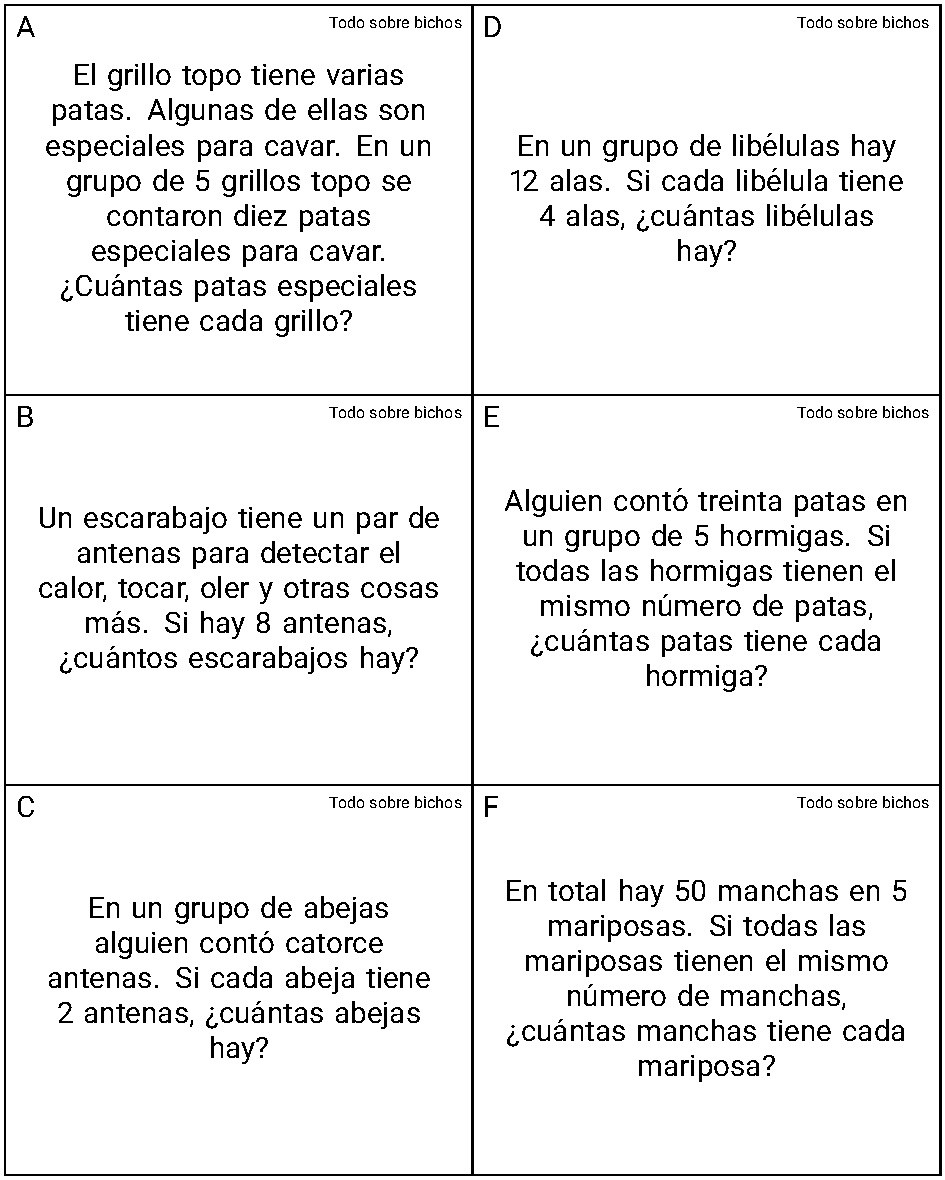
\includegraphics[max width=\linewidth, center]{external/tikz-source/todoSobreBichos-tarjetas.pdf}
% \end{image}%
\cleardoublepage
\end{subsubsectionptx}
%
%
\typeout{************************************************}
\typeout{Preguntas de comprensión  Actividad de cierre}
\typeout{************************************************}
%
\begin{reading-questions-subsubsection}{Preguntas de comprensión}{Actividad de cierre}{}{Actividad de cierre}{}{}{lec-escribamosExpresionesDivision-cool}
%
\end{reading-questions-subsubsection}
\end{subsectionptx}
%
%
\typeout{************************************************}
\typeout{Ejercicios  Problemas de práctica de la sección A}
\typeout{************************************************}
%
\begin{exercises-subsection}{Ejercicios}{Problemas de práctica de la sección A}{}{Problemas de práctica}{}{}{gra3-uni4-secA-ProblemasPractica}
%
%
%
%
%
%
%
%
%
%
%
%
\end{exercises-subsection}
\end{sectionptx}
%
%
\typeout{************************************************}
\typeout{Sección  Sección B -~Relacionemos la multiplicación y la división}
\typeout{************************************************}
%
\begin{sectionptx}{Sección}{Sección B -~Relacionemos la multiplicación y la división}{}{Sección B -~Relacionemos la multiplicación y la división}{}{}{gra3-uni4-secB}
%
%
\typeout{************************************************}
\typeout{Subsección  Lección 6 -~La división como un factor desconocido}
\typeout{************************************************}
%
\begin{subsectionptx}{Subsección}{Lección 6 -~La división como un factor desconocido}{}{Lección 6}{}{}{lec-divisionComoFactorDesconocido}
%
%
\typeout{************************************************}
\typeout{Subsubsección  Actividad 2}
\typeout{************************************************}
%
\begin{subsubsectionptx}{Subsubsección}{Actividad 2}{}{Actividad 2}{}{}{lec-divisionComoFactorDesconocido-act2}
\begin{activity}{Actividad}{En el mercado agrícola.}{act-enElMercadoAgricola}%
Completa cada fila. Prepárate para explicar tu razonamiento.%
\begin{image}{0}{1}{0}{}%
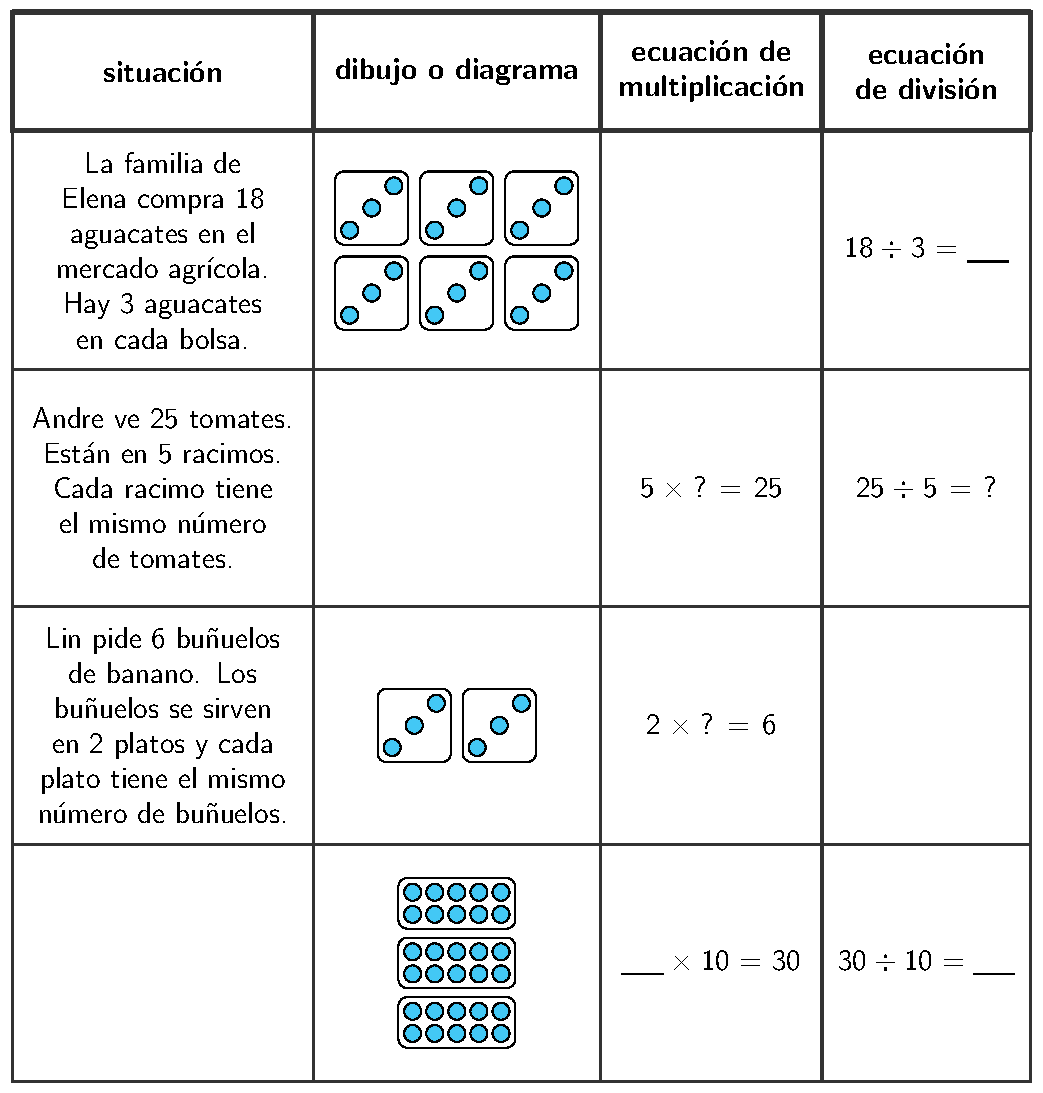
\includegraphics[max width=1.05\linewidth, center]{external/tikz-source/enElMercadoAgricola-blm-tab.pdf}
\end{image}%
\end{activity}%
\end{subsubsectionptx}
%
%
\typeout{************************************************}
\typeout{Preguntas de comprensión  Actividad de cierre}
\typeout{************************************************}
%
\begin{reading-questions-subsubsection}{Preguntas de comprensión}{Actividad de cierre}{}{Actividad de cierre}{}{}{lec-divisionComoFactorDesconocido-cool}
%
\end{reading-questions-subsubsection}
\end{subsectionptx}
%
%
\typeout{************************************************}
\typeout{Subsección  Lección 7 -~Relacionemos multiplicación y división}
\typeout{************************************************}
%
\begin{subsectionptx}{Subsección}{Lección 7 -~Relacionemos multiplicación y división}{}{Lección 7}{}{}{lec-relacionarMultiplicacionYDivision}
%
%
\typeout{************************************************}
\typeout{Subsubsección  Actividad 1}
\typeout{************************************************}
%
% \cleardoublepage
\begin{subsubsectionptx}{Subsubsección}{Actividad 1}{}{Actividad 1}{}{}{lec-relacionarMultiplicacionYDivision-act1}
\begin{activity}{Actividad}{Mesa redonda de división.}{act-mesaRedondaDeDivision}%
% En la siguiente tabla hay 4 recuadros. Tu profesor te pedirá que dibujes o escribas algo en cada uno.%
% \par
% Después de trabajar en cada recuadro, haz una pausa y espera que el profesor te dé las instrucciones para el siguiente recuadro.%
% %
% \begin{enumerate}
% \item{}Dibuja grupos iguales en el recuadro 1 de tu hoja de registro.%
% \item{}En el recuadro 2 de la hoja que acabaste de recibir, escribe una descripción de una situación de división que corresponda al dibujo.%
% \item{}En el recuadro 3 de la hoja que acabas de recibir, escribe una ecuación de multiplicación que corresponda al dibujo y a la situación de división. Usa un símbolo para representar la cantidad desconocida.%
% \item{}En el recuadro 4 de la hoja que acabas de recibir, escribe una ecuación de división que corresponda al dibujo, a la situación de división y a la ecuación de multiplicación. Usa un símbolo para representar la cantidad desconocida.%
% \end{enumerate}
\begin{image}{0}{1}{0}{}%
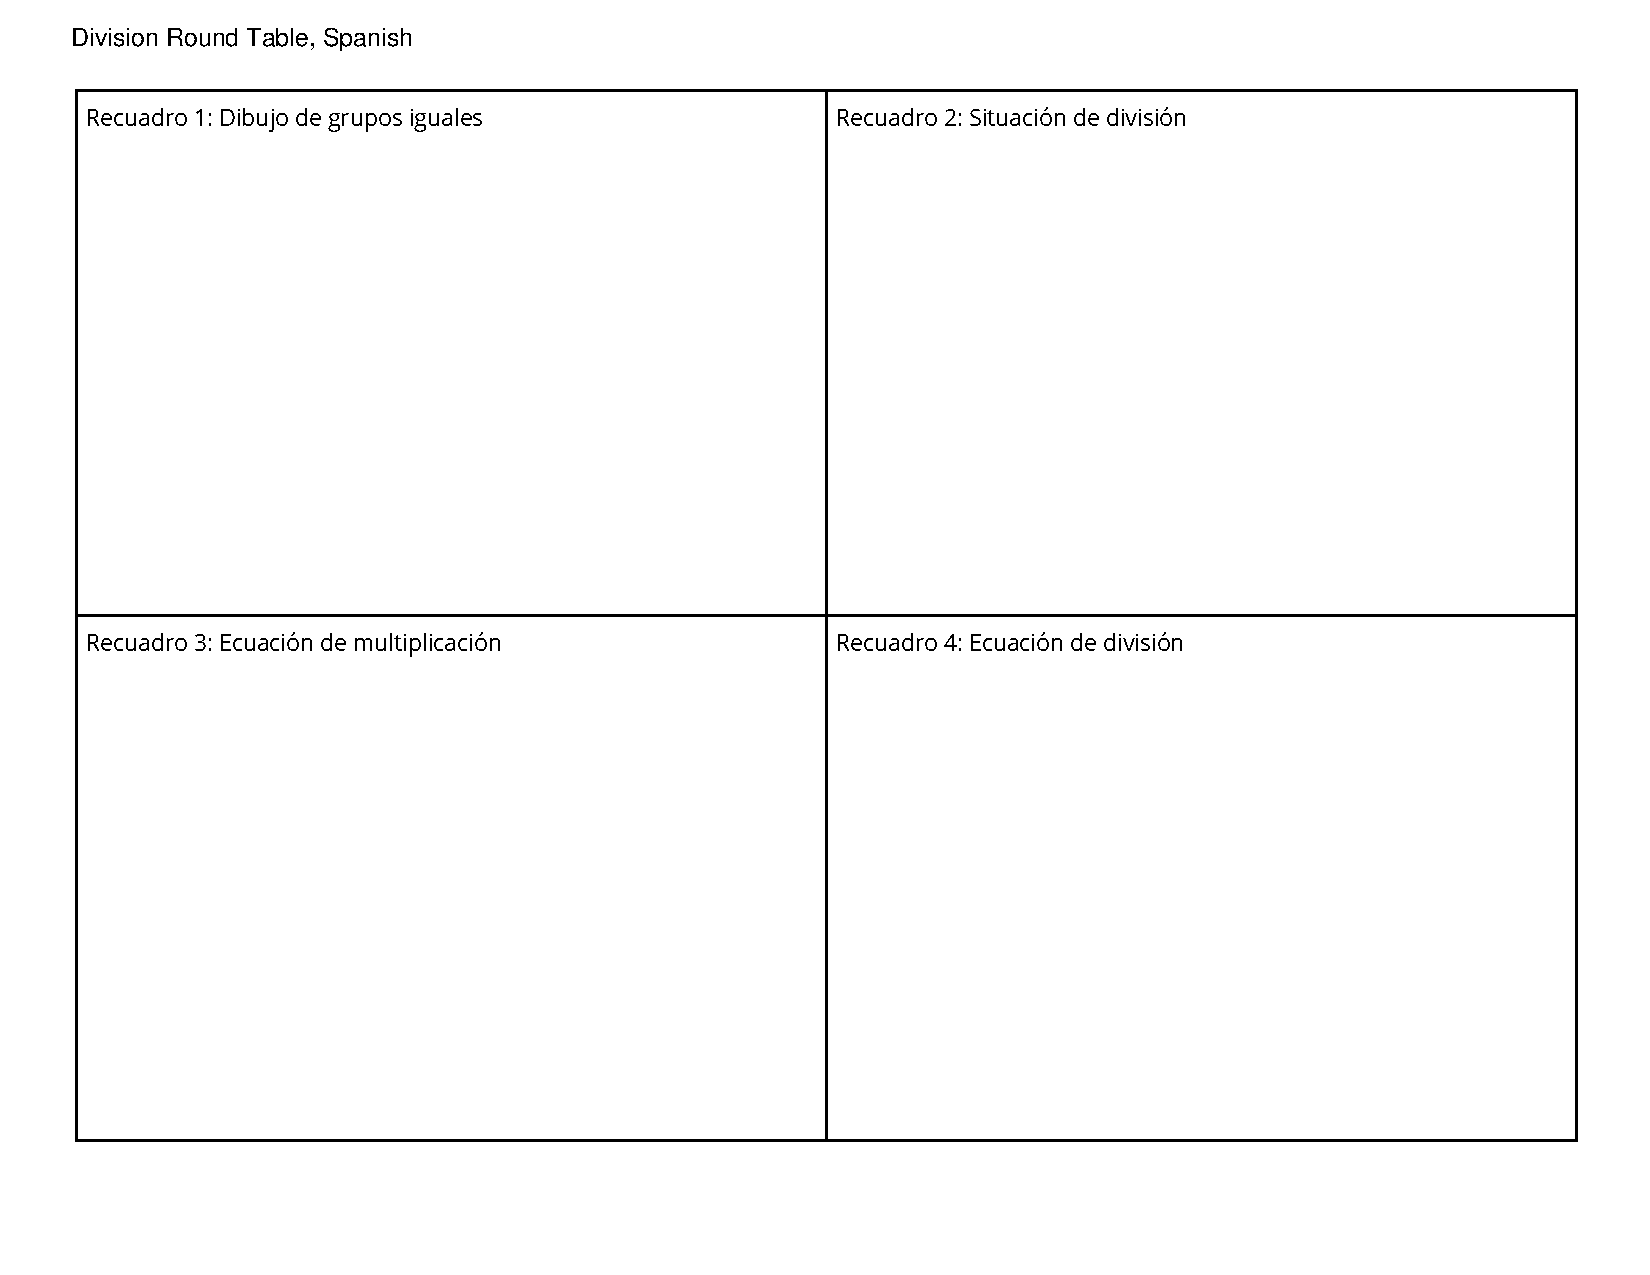
\includegraphics[trim=20 20 20 30, clip, width=1.3\linewidth,angle=90,origin=c]{external/blm/pdf-source/mesa-redonda-de-division.pdf}
\end{image}%
\end{activity}%
% \cleardoublepage
\end{subsubsectionptx}
%
%
\typeout{************************************************}
\typeout{Subsubsección  Actividad 2}
\typeout{************************************************}
%

%
%
\typeout{************************************************}
\typeout{Preguntas de comprensión  Actividad de cierre}
\typeout{************************************************}
%
\begin{reading-questions-subsubsection}{Preguntas de comprensión}{Actividad de cierre}{}{Actividad de cierre}{}{}{lec-relacionarMultiplicacionYDivision-cool}
%
\end{reading-questions-subsubsection}
\end{subsectionptx}
%
%
\typeout{************************************************}
\typeout{Subsección  Lección 8 -~Relacionemos cocientes con productos que nos sabemos}
\typeout{************************************************}
%
\begin{subsectionptx}{Subsección}{Lección 8 -~Relacionemos cocientes con productos que nos sabemos}{}{Lección 8}{}{}{lec-relCocientesProductos}
%
%
\typeout{************************************************}
\typeout{Subsubsección  Actividad 1}
\typeout{************************************************}
%
\begin{subsubsectionptx}{Subsubsección}{Actividad 1}{}{Actividad 1}{}{}{lec-relCocientesProductos-act1}
\begin{activity}{Actividad}{Clasificación de tarjetas: Multiplicación.}{act-clasificacionDeTarjetas-multiplicacion}%
Hazle preguntas a tu compañero sobre sus hechos de multiplicación. Clasifica los hechos de tu compañero en una de estas columnas:%
\begin{image}{0}{1}{0}{}%
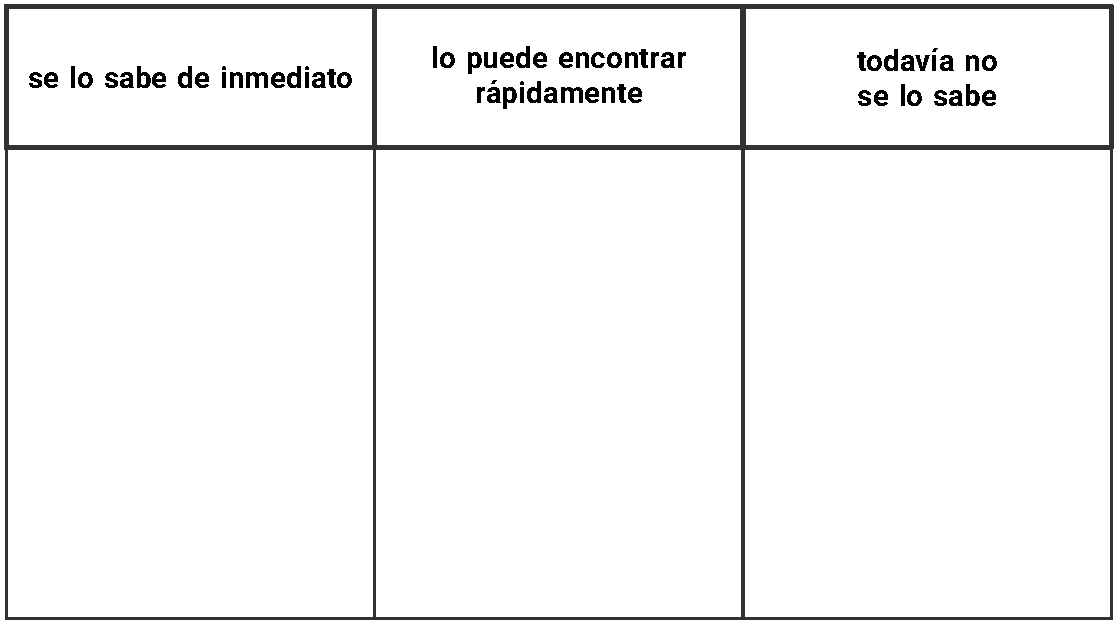
\includegraphics[max width=\linewidth, center]{external/tikz-source/clasificacionTarjetas-mult-paraBLM.pdf}
\end{image}%
Anota cinco expresiones de multiplicación que vas a practicar.%
%
\begin{enumerate}
\item{\vspace{0.5cm}}%
\item{\vspace{0.5cm}}%
\item{\vspace{0.5cm}}%
\item{\vspace{0.5cm}}%
\item{\vspace{0.5cm}}%
\end{enumerate}
\end{activity}%
\cleardoublepage
Tarjetas para recortar:
\par
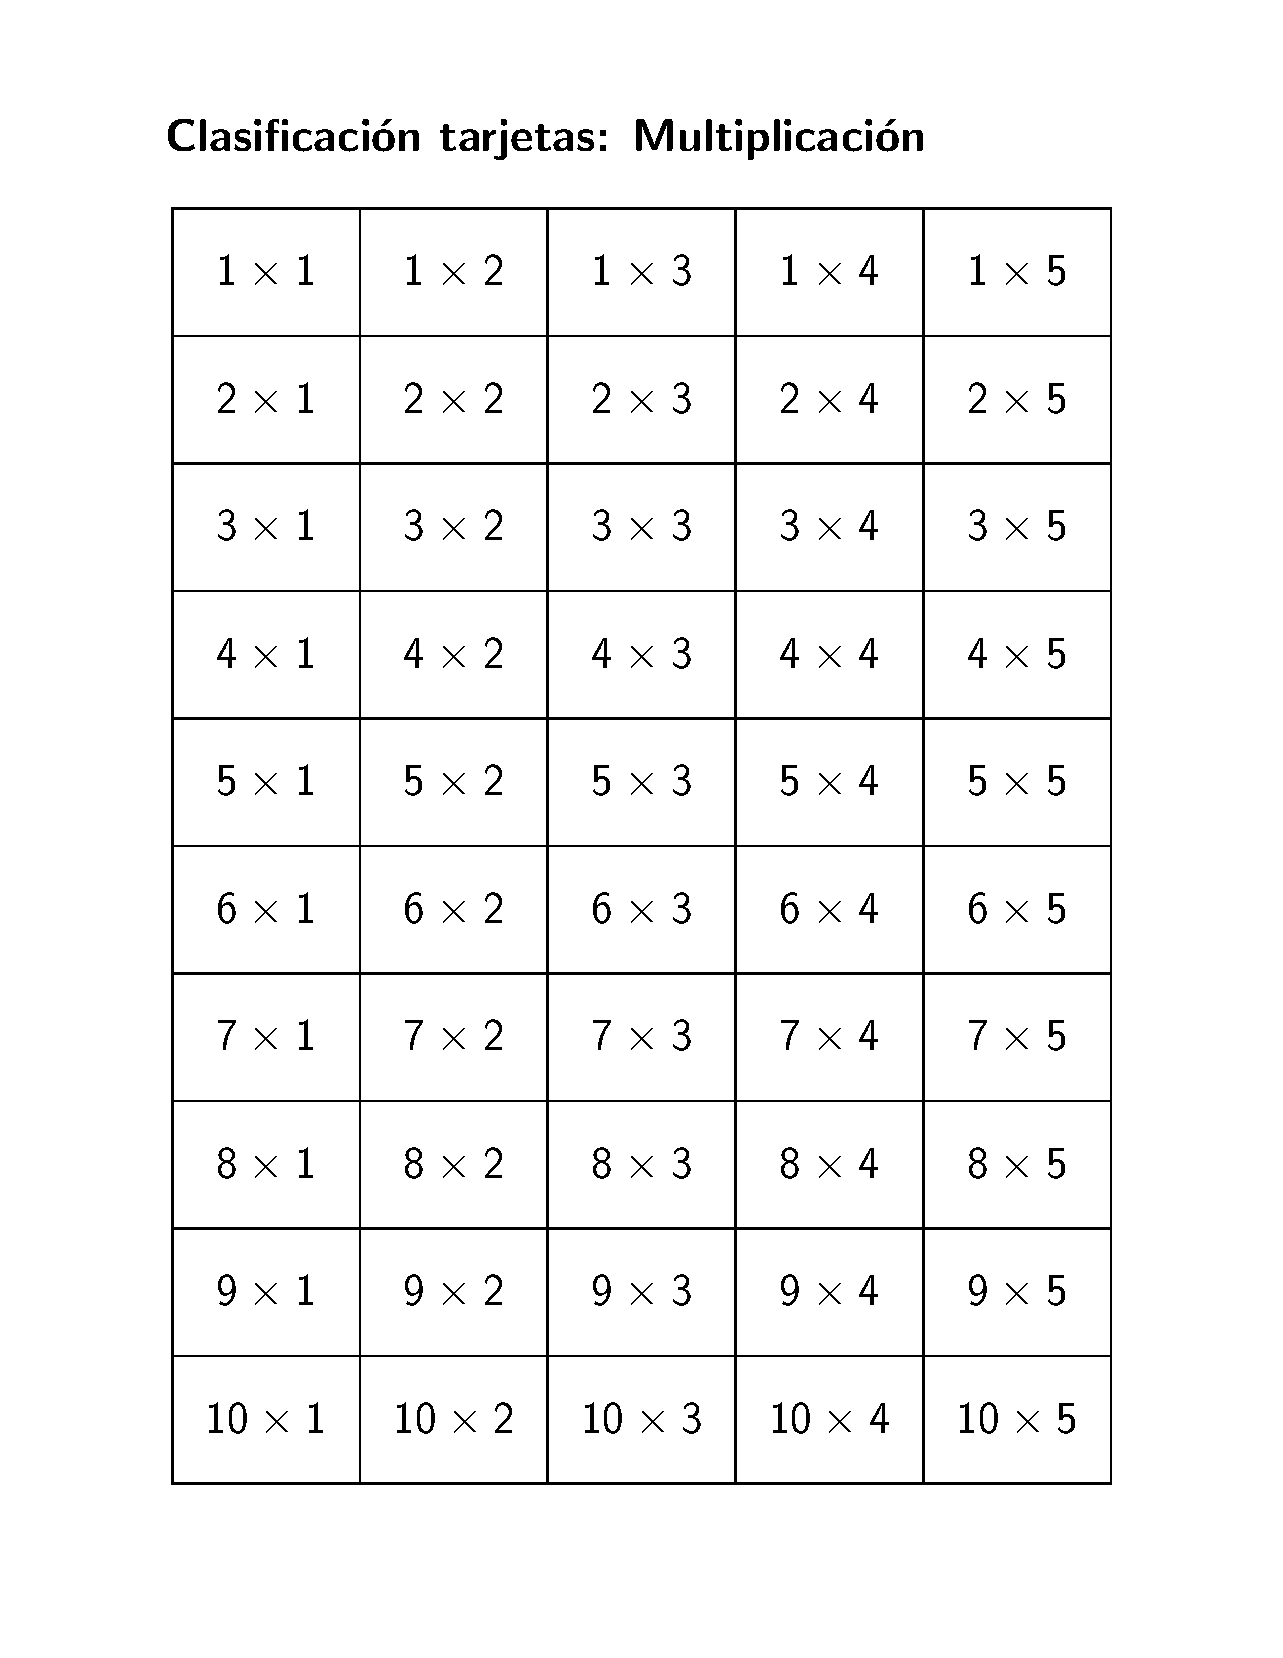
\includegraphics[page=1, trim=70 80 80 100,clip, width=1.05\linewidth]{external/blm/tikz-source/clasificacionTarjetas-multiplicacion-blm.pdf}

\cleardoublepage
Más tarjetas para recortar:
\par
\includegraphics[page=2, trim=70 80 80 100,clip, width=1.05\linewidth]{external/blm/tikz-source/clasificacionTarjetas-multiplicacion-blm.pdf}
\par
\cleardoublepage
\end{subsubsectionptx}
%
%
\typeout{************************************************}
\typeout{Subsubsección  Actividad 2}
\typeout{************************************************}
%
\begin{subsubsectionptx}{Subsubsección}{Actividad 2}{}{Actividad 2}{}{}{lec-relCocientesProductos-act2}
\begin{activity}{Actividad}{Si sé que \textellipsis{}, entonces sé que \textellipsis{}.}{act-siSeQueEntoncesSeQue}%
Si sé que \(4 \times 5 = 20\), entonces sé que \fillintext{10}.%
%
\begin{enumerate}
\item{}Coloquen las tarjetas de hechos de multiplicación en un montón, boca abajo.%
\item{}Por turnos, tomen una tarjeta de hechos de multiplicación.%
\item{}Usen el hecho de multiplicación de la tarjeta para escribir una ecuación de multiplicación en la columna “Si sé que \textellipsis{}”%
\item{}Después, anoten las ecuaciones de división relacionadas en la columna “Entonces sé que   \textellipsis{}”%
\end{enumerate}
\begin{image}{0}{1}{0}{}%
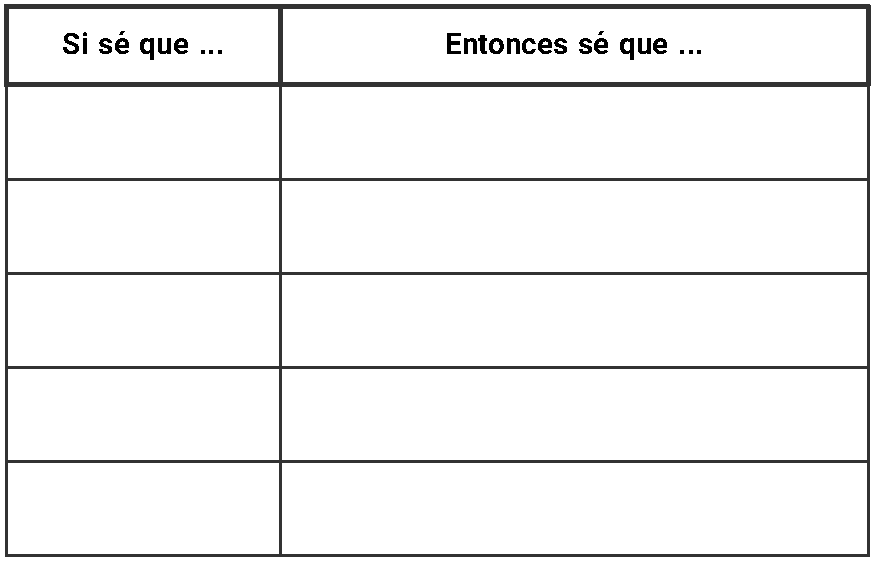
\includegraphics[max width=\linewidth, center]{external/tikz-source/siSeQueEntoncesSeQue-tab-libroTrabajo.pdf}
\end{image}%
\end{activity}%
\end{subsubsectionptx}
%
%
\typeout{************************************************}
\typeout{Preguntas de comprensión  Actividad de cierre}
\typeout{************************************************}
%
\begin{reading-questions-subsubsection}{Preguntas de comprensión}{Actividad de cierre}{}{Actividad de cierre}{}{}{lec-relCocientesProductos-cool}
%
\end{reading-questions-subsubsection}
\end{subsectionptx}
%
%
\typeout{************************************************}
\typeout{Subsección  Lección 9 -~Patrones en la tabla de multiplicar}
\typeout{************************************************}
%
\begin{subsectionptx}{Subsección}{Lección 9 -~Patrones en la tabla de multiplicar}{}{Lección 9}{}{}{lec-patronesTablaMultiplicar}
%
%
\typeout{************************************************}
\typeout{Subsubsección  Actividad 1}
\typeout{************************************************}
%

%
%
\typeout{************************************************}
\typeout{Subsubsección  Actividad 2}
\typeout{************************************************}
%
\clearpage
\begin{subsubsectionptx}{Subsubsección}{Actividad 2}{}{Actividad 2}{}{}{lec-patronesTablaMultiplicar-act2}
\begin{activity}{Actividad}{Si sé que \textellipsis{}, entonces sé que \textellipsis{}: Multiplicación.}{act-siSeQueEntoncesSeQueMult}%
%
\begin{enumerate}
\item{}En cada fila, escribe al menos dos hechos de multiplicación que puedes descifrar porque conoces el hecho de multiplicación dado en la columna de la izquierda. Prepárate para compartir tu razonamiento.%
\begin{image}{0}{1}{0}{}%
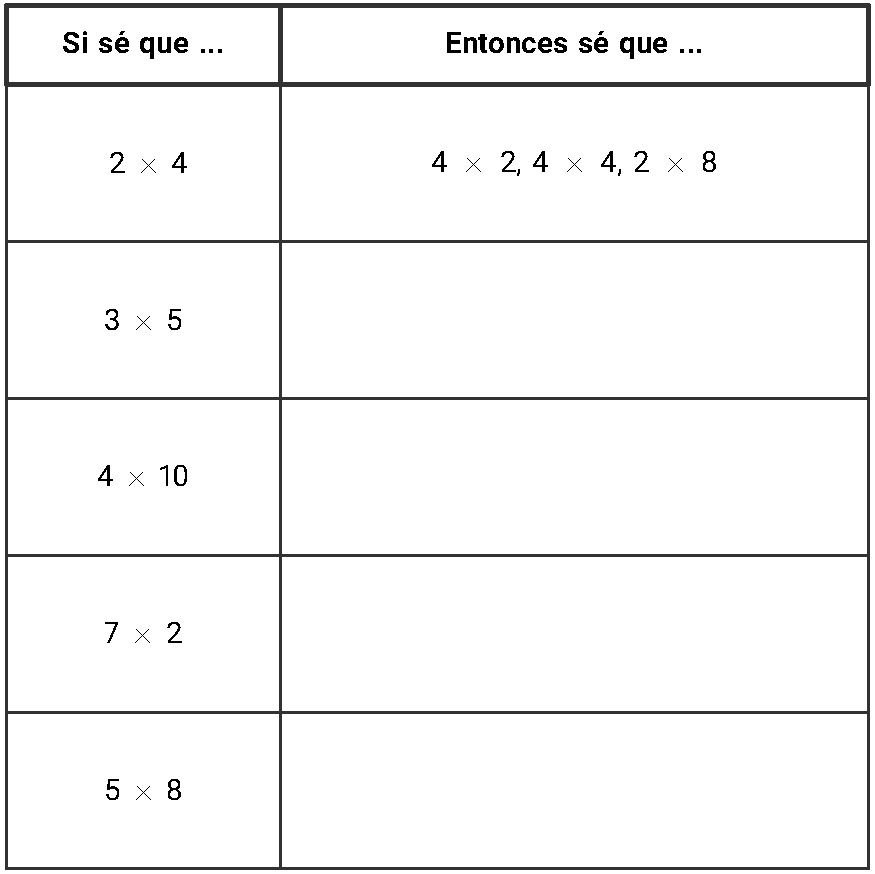
\includegraphics[max width=\linewidth, center]{external/tikz-source/siSeQueEntoncesSeQueMult-BLM-tab.pdf}
\end{image}%
\item{}Si te queda tiempo, completa el resto de la tabla de multiplicar. Usa los hechos de multiplicación que conoces para encontrar aquellos que no conoces.%
\end{enumerate}
\end{activity}%
\end{subsubsectionptx}
%
%
\typeout{************************************************}
\typeout{Preguntas de comprensión  Actividad de cierre}
\typeout{************************************************}
%
\begin{reading-questions-subsubsection}{Preguntas de comprensión}{Actividad de cierre}{}{Actividad de cierre}{}{}{lec-patronesTablaMultiplicar-cool}
%
\end{reading-questions-subsubsection}
\end{subsectionptx}
%
%
\typeout{************************************************}
\typeout{Subsección  Lección 10 -~Exploremos estrategias de multiplicación con rectángulos}
\typeout{************************************************}
%
\begin{subsectionptx}{Subsección}{Lección 10 -~Exploremos estrategias de multiplicación con rectángulos}{}{Lección 10}{}{}{lec-estrategiasMultConRectangulos}
%
%
\typeout{************************************************}
\typeout{Subsubsección  Actividad 1}
\typeout{************************************************}
%
\clearpage
\begin{subsubsectionptx}{Subsubsección}{Actividad 1}{}{Actividad 1}{}{}{lec-estrategiasMultConRectangulos-act1}
\begin{activity}{Actividad}{De diagramas a expresiones.}{act-deDiagramasAExpresiones}%
%
\begin{enumerate}
\item[2.] Este es otro rectángulo.%
\begin{image}{0}{1}{0}{}%
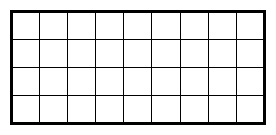
\includegraphics[max width=\linewidth, center]{external/svg-source/tikz-file-153048.pdf}
\end{image}%
Podemos encontrar su área hallando \(4 \times 9\).%
%
\begin{enumerate}
\item{}Marca o colorea el rectángulo de una manera que te ayude a encontrar su área.%
\item{}Escribe una o más expresiones que representen lo que hiciste en el diagrama y muestra cómo encontraste el área.%
% \begin{image}{0}{1}{0}{}%
% 
\includegraphics[max width=\linewidth, center]{external/whitespace-tikz/4cm.pdf}
% \end{image}%
\end{enumerate}
\end{enumerate}
\end{activity}%
\end{subsubsectionptx}
%
%
\typeout{************************************************}
\typeout{Subsubsección  Actividad 2}
\typeout{************************************************}
%
\begin{subsubsectionptx}{Subsubsección}{Actividad 2}{}{Actividad 2}{}{}{lec-estrategiasMultConRectangulos-act2}
\begin{activity}{Actividad}{De expresiones a diagramas.}{act-deExpresionesADiagramas}%
\begin{sidebyside}{3}{0.0166666666666667}{0.0166666666666667}{0.0333333333333333}%
\begin{sbspanel}{0.3}%
Noah%
\par
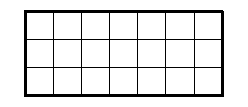
\includegraphics[max width=\linewidth, center]{external/svg-source/tikz-file-153051.pdf}
%
\begin{equation*}
(5\times 3)+(2 \times 3)
\end{equation*}
%
\end{sbspanel}%
\begin{sbspanel}{0.3}%
Priya%
\par
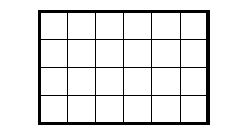
\includegraphics[max width=\linewidth, center]{external/svg-source/tikz-file-153053.pdf}
%
\begin{equation*}
2 \times (2 \times 6)
\end{equation*}
%
\end{sbspanel}%
\begin{sbspanel}{0.3}%
Tyler%
\par

\includegraphics[max width=\linewidth, center]{external/svg-source/tikz-file-153054.pdf}
%
\begin{equation*}
(5 \times 8) + (3 \times 8)
\end{equation*}
%
\end{sbspanel}%
\end{sidebyside}%
\par
En cada rectángulo:%
%
\begin{enumerate}
\item{}Escribe los dos factores que se pueden multiplicar para encontrar su área.%
\item{}Marca o colorea cada rectángulo para mostrar la manera en la que cada estudiante vio el área. Prepárate para explicar tu razonamiento.%
\begin{image}{0}{1}{0}{}%

\includegraphics[max width=\linewidth, center]{external/whitespace-tikz/1cm.pdf}
\end{image}%
\end{enumerate}
\end{activity}%
\end{subsubsectionptx}
%
%
\typeout{************************************************}
\typeout{Preguntas de comprensión  Actividad de cierre}
\typeout{************************************************}
%
\begin{reading-questions-subsubsection}{Preguntas de comprensión}{Actividad de cierre}{}{Actividad de cierre}{}{}{lec-estrategiasMultConRectangulos-cool}
%
\end{reading-questions-subsubsection}
\end{subsectionptx}
%
%
\typeout{************************************************}
\typeout{Subsección  Lección 11 -~Estrategias de multiplicación para rectángulos sin cuadrícula}
\typeout{************************************************}
%
\begin{subsectionptx}{Subsección}{Lección 11 -~Estrategias de multiplicación para rectángulos sin cuadrícula}{}{Lección 11}{}{}{lec-estrategiasMultRectangulosSinCuadricula}
%
%
\typeout{************************************************}
\typeout{Subsubsección  Actividad 1}
\typeout{************************************************}
%
\begin{subsubsectionptx}{Subsubsección}{Actividad 1}{}{Actividad 1}{}{}{gra3-uni4-secB-lec11-act1}
\begin{activity}{Actividad}{Marca y después expresa.}{act-marcaDespuesExpresa}%
En cada caso:%
%
\begin{itemize}[label=\textbullet]
\item{}Marca o colorea cada rectángulo para mostrar una estrategia que ayude a encontrar su área.%
\item{}Escribe una o más expresiones que representen cómo encuentras el área.%
\end{itemize}
\begin{sidebyside}{3}{0}{0}{0}%
\begin{sbspanel}{0.391}%
A%
\par
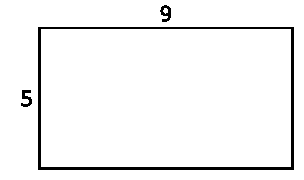
\includegraphics[max width=\linewidth, center]{external/svg-source/tikz-file-153084.pdf}
\end{sbspanel}%
\begin{sbspanel}{0.261}%
B%
\par
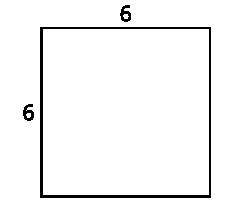
\includegraphics[max width=\linewidth, center]{external/svg-source/tikz-file-153085.pdf}
\end{sbspanel}%
\begin{sbspanel}{0.348}%
C%
\par
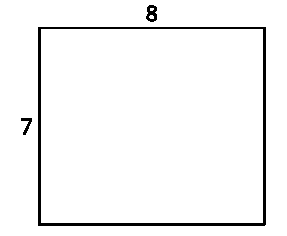
\includegraphics[max width=\linewidth, center]{external/svg-source/tikz-file-153086.pdf}
\end{sbspanel}%
\end{sidebyside}%
\begin{image}{0}{1}{0}{}%

\includegraphics[max width=\linewidth, center]{external/whitespace-tikz/2cm.pdf}
\end{image}%
\end{activity}%
\end{subsubsectionptx}
%
%
\typeout{************************************************}
\typeout{Subsubsección  Actividad 2}
\typeout{************************************************}
%
\begin{subsubsectionptx}{Subsubsección}{Actividad 2}{}{Actividad 2}{}{}{gra3-uni4-secB-lec11-act2}
\begin{activity}{Actividad}{Clasificación de tarjetas: Expresiones diferentes, mismo rectángulo.}{act-clasificacionDeTarjetas-expresionesMultiplicacionRectangulos}%
Las tarjetas para recortar tienen expresiones que representan áreas de rectángulos.%
\par
Clasifica las expresiones en grupos de manera que las expresiones de cada grupo representen el área del mismo rectángulo. Prepárate para explicar tu razonamiento.%
\par
Si te ayuda, puedes dibujar rectángulos.%
\end{activity}%
\cleardoublepage
Tarjetas para recortar:
\begin{image}{0}{1}{0}{}%
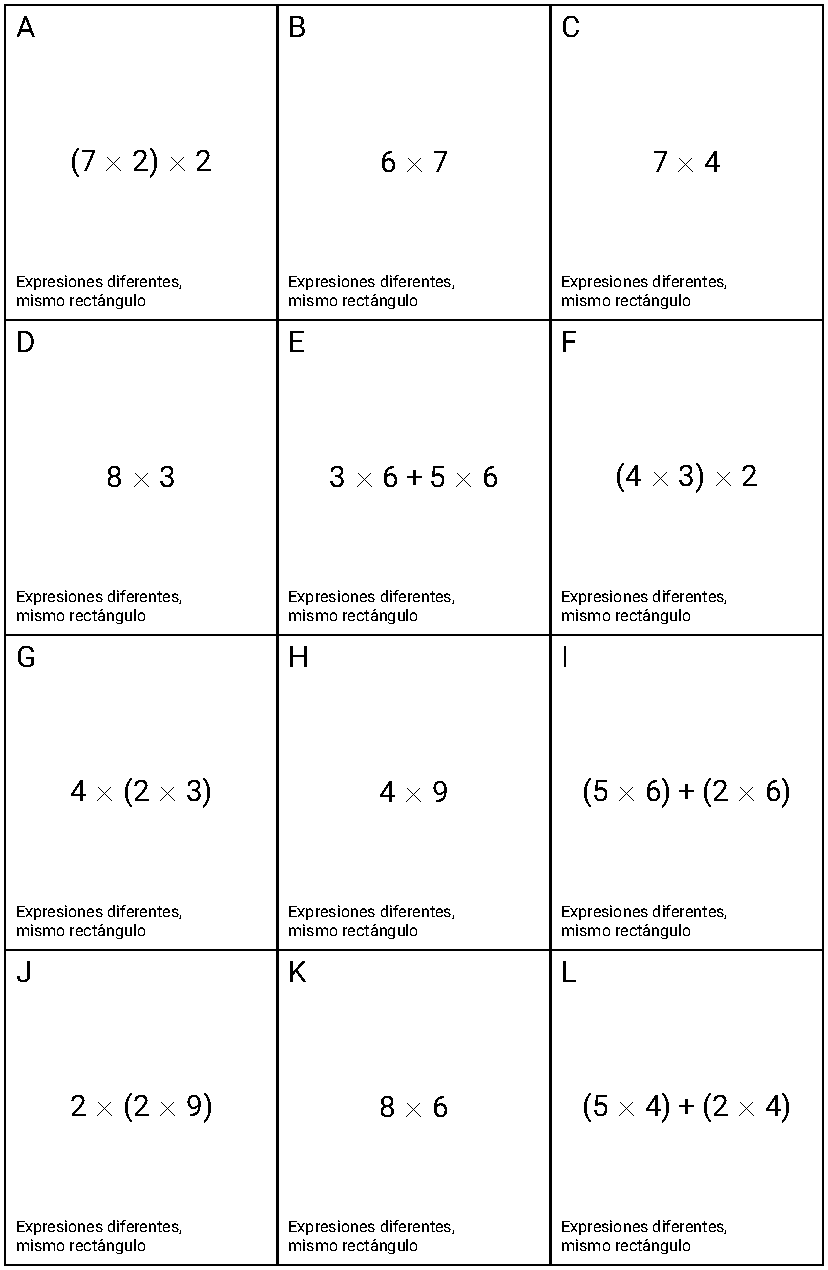
\includegraphics[max width=\linewidth, center]{external/blm/tikz-source/clasificacionTarjetas-expresionesDiferentesMismoRect-tarjetas.pdf}
\end{image}
\cleardoublepage
\end{subsubsectionptx}
%
%
\typeout{************************************************}
\typeout{Preguntas de comprensión  Actividad de cierre}
\typeout{************************************************}
%
\begin{reading-questions-subsubsection}{Preguntas de comprensión}{Actividad de cierre}{}{Actividad de cierre}{}{}{gra3-uni4-secB-lec11-cool}
%
\end{reading-questions-subsubsection}
\end{subsectionptx}
%
%
\typeout{************************************************}
\typeout{Ejercicios  Problemas de práctica de la sección B}
\typeout{************************************************}
%
\begin{exercises-subsection}{Ejercicios}{Problemas de práctica de la sección B}{}{Problemas de práctica}{}{}{gra3-uni4-secB-ProblemasPractica}
%
%
%
%
%
%
%
\end{exercises-subsection}
\end{sectionptx}
%
%
\typeout{************************************************}
\typeout{Sección  Sección C -~Multipliquemos números más grandes}
\typeout{************************************************}
%
\begin{sectionptx}{Sección}{Sección C -~Multipliquemos números más grandes}{}{Sección C -~Multipliquemos números más grandes}{}{}{gra3-uni4-secC}
%
%
\typeout{************************************************}
\typeout{Subsección  Lección 12 -~Multipliquemos múltiplos de diez}
\typeout{************************************************}
%
\begin{subsectionptx}{Subsección}{Lección 12 -~Multipliquemos múltiplos de diez}{}{Lección 12}{}{}{lec-multiplicarMultiplos10}
%
%
\typeout{************************************************}
\typeout{Subsubsección  Actividad 1}
\typeout{************************************************}
%
\begin{subsubsectionptx}{Subsubsección}{Actividad 1}{}{Actividad 1}{}{}{lec-multiplicarMultiplos10-act1}
\begin{activity}{Actividad}{Una gran cantidad de dólares.}{act-granCantidadDolares}%
Seis amigos juegan un juego de mesa en el que se usa dinero de juguete. Hay billetes de papel de \textdollar{}5, \textdollar{}10, \textdollar{}20, \textdollar{}50 y de \textdollar{}100.%
%
\begin{enumerate}
\item{}Cada jugador recibió \textdollar{}100 para empezar. ¿Cuáles de los siguientes podrían ser los billetes que recibió cada jugador?%
\par
Escribe una expresión que represente los billetes de juguete y escribe la cantidad de dólares.%
\begin{image}{0}{1}{0}{}%
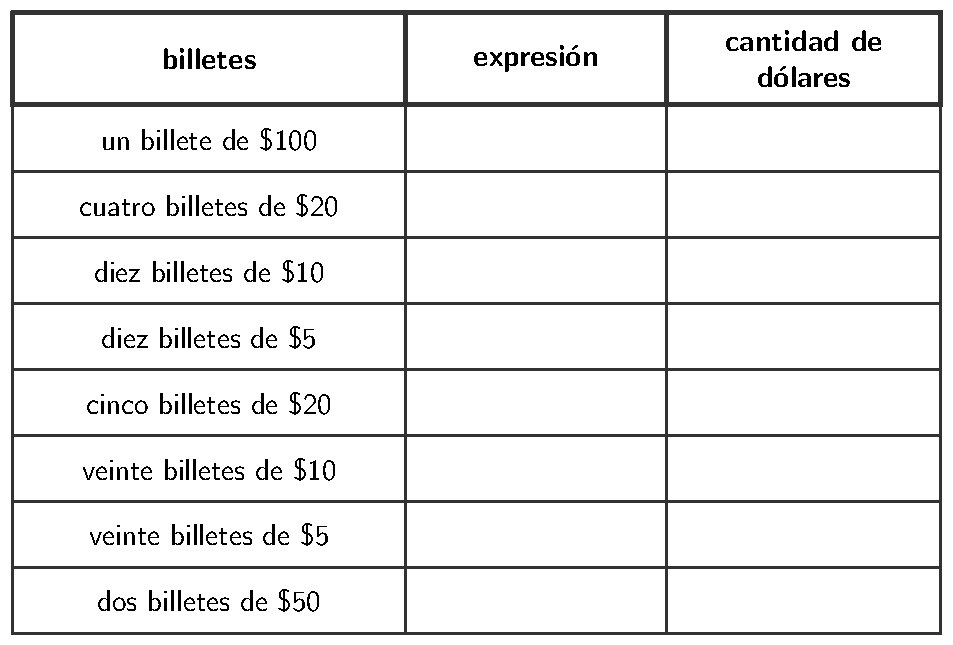
\includegraphics[max width=\linewidth, center]{external/tikz-source/unaGranCantidadDeDolares-tab1.pdf}
\end{image}%
\item{}En un momento del juego, Noah tuvo que pagarle a Lin \textdollar{}150. Él le dio esa cantidad usando billetes del mismo tipo.%
%
\begin{enumerate}
\item{}¿Cuáles y cuántos billetes podría haber usado Noah para completar \textdollar{}150? Nombra todas las posibilidades.%
\begin{image}{0}{1}{0}{}%

\includegraphics[max width=\linewidth, center]{external/whitespace-tikz/1cm.pdf}
\end{image}%
\item{}Escribe una expresión para cada forma en la que Noah podría haberle pagado a Lin.%
% \begin{image}{0}{1}{0}{}%
% 
\includegraphics[max width=\linewidth, center]{external/whitespace-tikz/1cm.pdf}
% \end{image}%
\end{enumerate}
\clearpage
\item{}La tabla muestra lo que tenían los jugadores al final del juego. Gana la persona que tenga la mayor cantidad de dinero. ¿Quién ganó el juego?%
\par
Escribe una expresión que represente los billetes que tiene cada persona y escribe la cantidad de dólares.%
\begin{image}{0}{1}{0}{}%
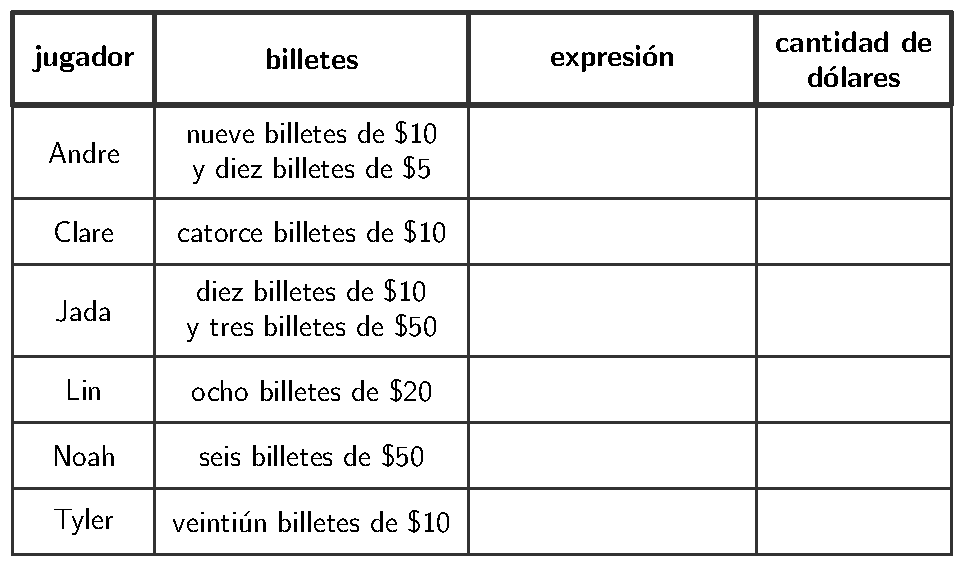
\includegraphics[max width=\linewidth, center]{external/tikz-source/unaGranCantidadDeDolares-tab2.pdf}
\end{image}%
\end{enumerate}
\end{activity}%
\end{subsubsectionptx}
%
%
\typeout{************************************************}
\typeout{Preguntas de comprensión  Actividad de cierre}
\typeout{************************************************}
%
\begin{reading-questions-subsubsection}{Preguntas de comprensión}{Actividad de cierre}{}{Actividad de cierre}{}{}{lec-multiplicarMultiplos10-cool}
%
\end{reading-questions-subsubsection}
\end{subsectionptx}
%
%
\typeout{************************************************}
\typeout{Subsección  Lección 13 -~Resolvamos problemas de grupos iguales}
\typeout{************************************************}
%
\begin{subsectionptx}{Subsección}{Lección 13 -~Resolvamos problemas de grupos iguales}{}{Lección 13}{}{}{lec-problemasMult11a19}
%
%
%
%
\typeout{************************************************}
\typeout{Preguntas de comprensión  Actividad de cierre}
\typeout{************************************************}
%
\begin{reading-questions-subsubsection}{Preguntas de comprensión}{Actividad de cierre}{}{Actividad de cierre}{}{}{lec-problemasMult11a19-cool}
%
\end{reading-questions-subsubsection}
\end{subsectionptx}
%
%
\typeout{************************************************}
\typeout{Subsección  Lección 14 -~Formas de representar la multiplicación de números del 11 al 19}
\typeout{************************************************}
%
\begin{subsectionptx}{Subsección}{Lección 14 -~Formas de representar la multiplicación de números del 11 al 19}{}{Lección 14}{}{}{lec-representarMultiplicacion11a19}
%
%
\typeout{************************************************}
\typeout{Preguntas de comprensión  Actividad de cierre}
\typeout{************************************************}
%
\begin{reading-questions-subsubsection-numberless}{Preguntas de comprensión}{Actividad de cierre}{}{Actividad de cierre}{}{}{lec-representarMultiplicacion11a19-cool}
%
\end{reading-questions-subsubsection-numberless}
\end{subsectionptx}
%
%
\typeout{************************************************}
\typeout{Subsección  Lección 15 -~Grupos iguales, números más grandes}
\typeout{************************************************}
%
\begin{subsectionptx}{Subsección}{Lección 15 -~Grupos iguales, números más grandes}{}{Lección 15}{}{}{lec-problemasMult11a19MasGrandes}
%
%
\typeout{************************************************}
\typeout{Preguntas de comprensión  Actividad de cierre}
\typeout{************************************************}
%
\begin{reading-questions-subsubsection-numberless}{Preguntas de comprensión}{Actividad de cierre}{}{Actividad de cierre}{}{}{lec-problemasMult11a19MasGrandes-cool}
%
\end{reading-questions-subsubsection-numberless}
\end{subsectionptx}
%
%
\typeout{************************************************}
\typeout{Subsección  Lección 16 -~Multipliquemos números más grandes que 20}
\typeout{************************************************}
%
\begin{subsectionptx}{Subsección}{Lección 16 -~Multipliquemos números más grandes que 20}{}{Lección 16}{}{}{lec-multiplicarNumsMayoresA20}
%
%
\typeout{************************************************}
\typeout{Subsubsección  Actividad 3}
\typeout{************************************************}
%
\clearpage
\begin{subsubsectionptx}{Subsubsección}{Actividad 3}{}{Actividad 3}{}{}{lec-multiplicarNumsMayoresA20-act3}
\begin{activity}{Actividad}{Juguemos “Cerca de 100, multiplicación” (opcional).}{act-juegoCerca100Multiplicacion}%
Tarjetas para recortar en las siguiente páginas.%
% %
% \begin{enumerate}
% \item{}Pon las tarjetas boca abajo.%
% \item{}Cada jugador toma 4 tarjetas.%
% \item{}Cada jugador escoge 2 de sus tarjetas para completar la expresión y hacer que el valor esté lo más cerca posible de 100. Escribe los 2 dígitos y el producto.%
% \item{}El jugador que esté más cerca de 100, gana esa ronda.%
% \item{}Juega 5 rondas. El jugador que gane la mayoría de rondas, gana la partida.%
% \end{enumerate}
\begin{sidebyside}{2}{0}{0}{0.1}%
\begin{sbspanel}{0.45}%
\alert{Partida 1}%
\end{sbspanel}%
\begin{sbspanel}{0.45}%
\par
\alert{Partida 2}%
\end{sbspanel}%
\end{sidebyside}%
\begin{sidebyside}{2}{0}{0}{0.1}%
\begin{sbspanel}{0.45}%
Ronda 1%
\par
%
\begin{equation*}
\boxed{\phantom{\frac{00}{00}}} \times 1 \ \boxed{\phantom{\frac{00}{00}}}= \underline{\hspace{1cm}}
\end{equation*}
%
\end{sbspanel}%
\begin{sbspanel}{0.45}%
Ronda 1%
\par
%
\begin{equation*}
\boxed{\phantom{\frac{00}{00}}} \times 2 \ \boxed{\phantom{\frac{00}{00}}}= \underline{\hspace{1cm}}
\end{equation*}
%
\end{sbspanel}%
\end{sidebyside}%
\begin{sidebyside}{2}{0}{0}{0.1}%
\begin{sbspanel}{0.45}%
Ronda 2%
\par
%
\begin{equation*}
\boxed{\phantom{\frac{00}{00}}} \times 1 \ \boxed{\phantom{\frac{00}{00}}}= \underline{\hspace{1cm}}
\end{equation*}
%
\end{sbspanel}%
\begin{sbspanel}{0.45}%
Ronda 2%
\par
%
\begin{equation*}
\boxed{\phantom{\frac{00}{00}}} \times 2 \ \boxed{\phantom{\frac{00}{00}}}= \underline{\hspace{1cm}}
\end{equation*}
%
\end{sbspanel}%
\end{sidebyside}%
\begin{sidebyside}{2}{0}{0}{0.1}%
\begin{sbspanel}{0.45}%
Ronda 3%
\par
%
\begin{equation*}
\boxed{\phantom{\frac{00}{00}}} \times 1 \ \boxed{\phantom{\frac{00}{00}}}= \underline{\hspace{1cm}}
\end{equation*}
%
\end{sbspanel}%
\begin{sbspanel}{0.45}%
Ronda 3%
\par
%
\begin{equation*}
\boxed{\phantom{\frac{00}{00}}} \times 2 \ \boxed{\phantom{\frac{00}{00}}}= \underline{\hspace{1cm}}
\end{equation*}
%
\end{sbspanel}%
\end{sidebyside}%
\begin{sidebyside}{2}{0}{0}{0.1}%
\begin{sbspanel}{0.45}%
Ronda 4%
\par
%
\begin{equation*}
\boxed{\phantom{\frac{00}{00}}} \times 1 \ \boxed{\phantom{\frac{00}{00}}}= \underline{\hspace{1cm}}
\end{equation*}
%
\end{sbspanel}%
\begin{sbspanel}{0.45}%
Ronda 4%
\par
%
\begin{equation*}
\boxed{\phantom{\frac{00}{00}}} \times 2 \ \boxed{\phantom{\frac{00}{00}}}= \underline{\hspace{1cm}}
\end{equation*}
%
\end{sbspanel}%
\end{sidebyside}%
\begin{sidebyside}{2}{0}{0}{0.1}%
\begin{sbspanel}{0.45}%
Ronda 5%
\par
%
\begin{equation*}
\boxed{\phantom{\frac{00}{00}}} \times 1 \ \boxed{\phantom{\frac{00}{00}}}= \underline{\hspace{1cm}}
\end{equation*}
%
\end{sbspanel}%
\begin{sbspanel}{0.45}%
Ronda 5%
\par
%
\begin{equation*}
\boxed{\phantom{\frac{00}{00}}} \times 2 \ \boxed{\phantom{\frac{00}{00}}}= \underline{\hspace{1cm}}
\end{equation*}
%
\end{sbspanel}%
\end{sidebyside}%
%
\end{activity}%
\cleardoublepage
Tarjetas para recortar:
\begin{image}{0}{1}{0}{}%
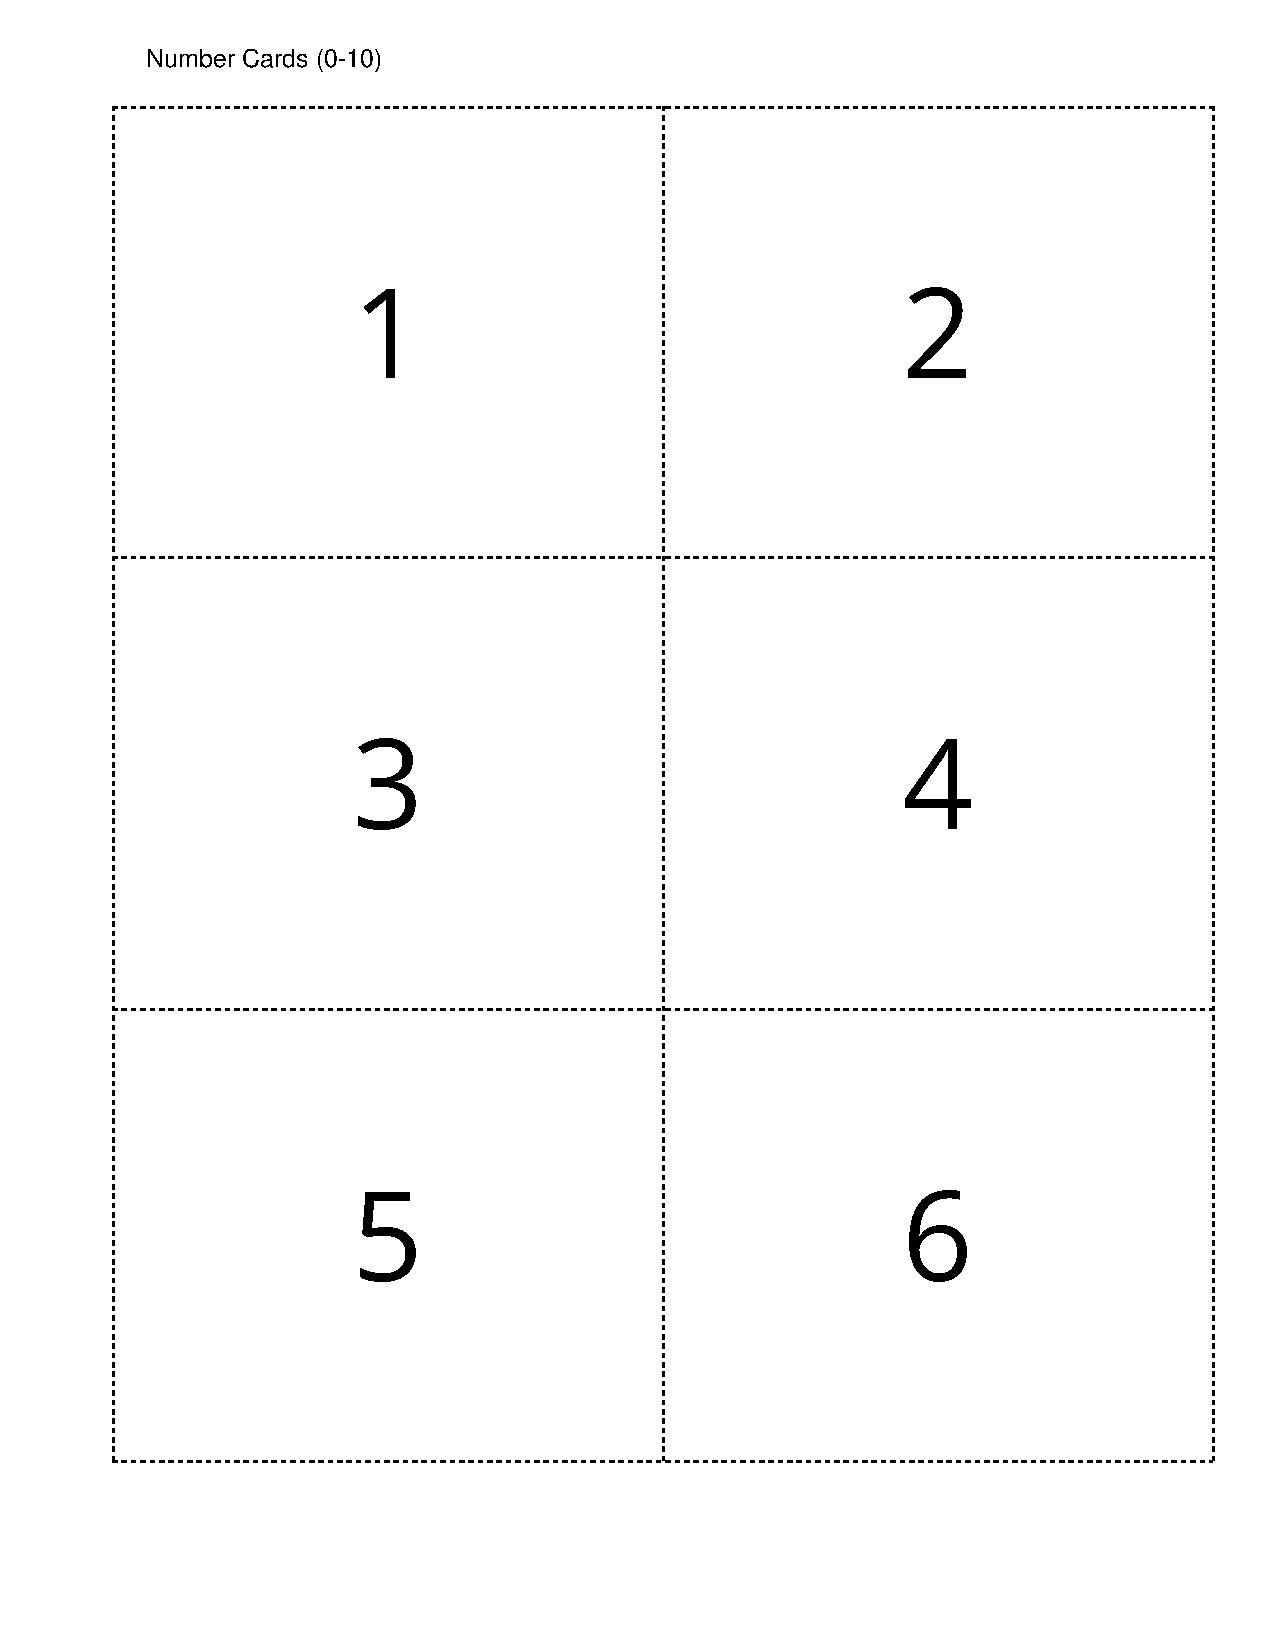
\includegraphics[page=1, rotate=90, scale=0.55, trim=40 40 20 40, clip, center] {external/blm/pdf-source/tarjetasDeDigitos.pdf}
\end{image}%
\begin{image}{0}{1}{0}{}%
\includegraphics[page=2, rotate=90, scale=0.55, trim=40 40 20 40, clip, center] {external/blm/pdf-source/tarjetasDeDigitos.pdf}
\end{image}%
\cleardoublepage
Tarjetas para recortar:
\begin{image}{0}{1}{0}{}%
\includegraphics[page=3, rotate=90, scale=0.55, trim=40 40 20 40, clip, center] {external/blm/pdf-source/tarjetasDeDigitos.pdf}
\end{image}%
\begin{image}{0}{1}{0}{}%
\includegraphics[page=4, rotate=90, scale=0.55, trim=40 40 20 40, clip, center] {external/blm/pdf-source/tarjetasDeDigitos.pdf}
\end{image}
% \cleardoublepage
\end{subsubsectionptx}
%
%
\typeout{************************************************}
\typeout{Preguntas de comprensión  Actividad de cierre}
\typeout{************************************************}
%
\begin{reading-questions-subsubsection}{Preguntas de comprensión}{Actividad de cierre}{}{Actividad de cierre}{}{}{lec-multiplicarNumsMayoresA20-cool}
%
\end{reading-questions-subsubsection}
\end{subsectionptx}
%
%
\typeout{************************************************}
\typeout{Subsección  Lección 17 -~Usemos las cuatro operaciones para resolver problemas}
\typeout{************************************************}
%
\begin{subsectionptx}{Subsección}{Lección 17 -~Usemos las cuatro operaciones para resolver problemas}{}{Lección 17}{}{}{lec-problemasCuatroOperaciones}
%
%
\typeout{************************************************}
\typeout{Preguntas de comprensión  Actividad de cierre}
\typeout{************************************************}
%
\begin{reading-questions-subsubsection-numberless}{Preguntas de comprensión}{Actividad de cierre}{}{Actividad de cierre}{}{}{lec-problemasCuatroOperaciones-cool}
%
\end{reading-questions-subsubsection-numberless}
\end{subsectionptx}
%
%
\typeout{************************************************}
\typeout{Ejercicios  Problemas de práctica de la sección C}
\typeout{************************************************}
%
\begin{exercises-subsection}{Ejercicios}{Problemas de práctica de la sección C}{}{Problemas de práctica}{}{}{gra3-uni4-secC-ProblemasPractica}
%
%

\end{exercises-subsection}
\end{sectionptx}
%
%
\typeout{************************************************}
\typeout{Sección  Sección D -~Dividamos números más grandes}
\typeout{************************************************}
%
\begin{sectionptx}{Sección}{Sección D -~Dividamos números más grandes}{}{Sección D -~Dividamos números más grandes}{}{}{gra3-uni4-secD}
%
%
\typeout{************************************************}
\typeout{Subsección  Lección 18 -~Números más grandes en grupos iguales}
\typeout{************************************************}
%
\begin{subsectionptx}{Subsección}{Lección 18 -~Números más grandes en grupos iguales}{}{Lección 18}{}{}{lec-gruposIgualesMasGrandes}
%
%
\typeout{************************************************}
\typeout{Preguntas de comprensión  Actividad de cierre}
\typeout{************************************************}
%
\begin{reading-questions-subsubsection-numberless}{Preguntas de comprensión}{Actividad de cierre}{}{Actividad de cierre}{}{}{lec-gruposIgualesMasGrandes-cool}
%
\end{reading-questions-subsubsection-numberless}
\end{subsectionptx}
%
%
\typeout{************************************************}
\typeout{Subsección  Lección 19 -~Formas de dividir números más grandes}
\typeout{************************************************}
%
\begin{subsectionptx}{Subsección}{Lección 19 -~Formas de dividir números más grandes}{}{Lección 19}{}{}{lec-formasDividirNumerosMasGrandes}
%
%
\typeout{************************************************}
\typeout{Preguntas de comprensión  Actividad de cierre}
\typeout{************************************************}
%
\begin{reading-questions-subsubsection-numberless}{Preguntas de comprensión}{Actividad de cierre}{}{Actividad de cierre}{}{}{lec-formasDividirNumerosMasGrandes-cool}
%
\end{reading-questions-subsubsection-numberless}
\end{subsectionptx}
%
%
\typeout{************************************************}
\typeout{Subsección  Lección 20 -~Estrategias para dividir}
\typeout{************************************************}
%
\begin{subsectionptx}{Subsección}{Lección 20 -~Estrategias para dividir}{}{Lección 20}{}{}{lec-estrategiasDividir}
%
%
\typeout{************************************************}
\typeout{Subsubsección  Actividad 3}
\typeout{************************************************}
%
\cleardoublepage
\begin{subsubsectionptx}{Subsubsección}{Actividad 3}{}{Actividad 3}{}{}{lec-estrategiasDividir-act3}
\begin{activity}{Actividad}{“Compara: Divide hasta 100” [OPCIONAL].}{act-comparaDivideHasta100}%
Tarjetas para recortar%
\end{activity}%
% \begin{image}{0}{1}{0}{}%
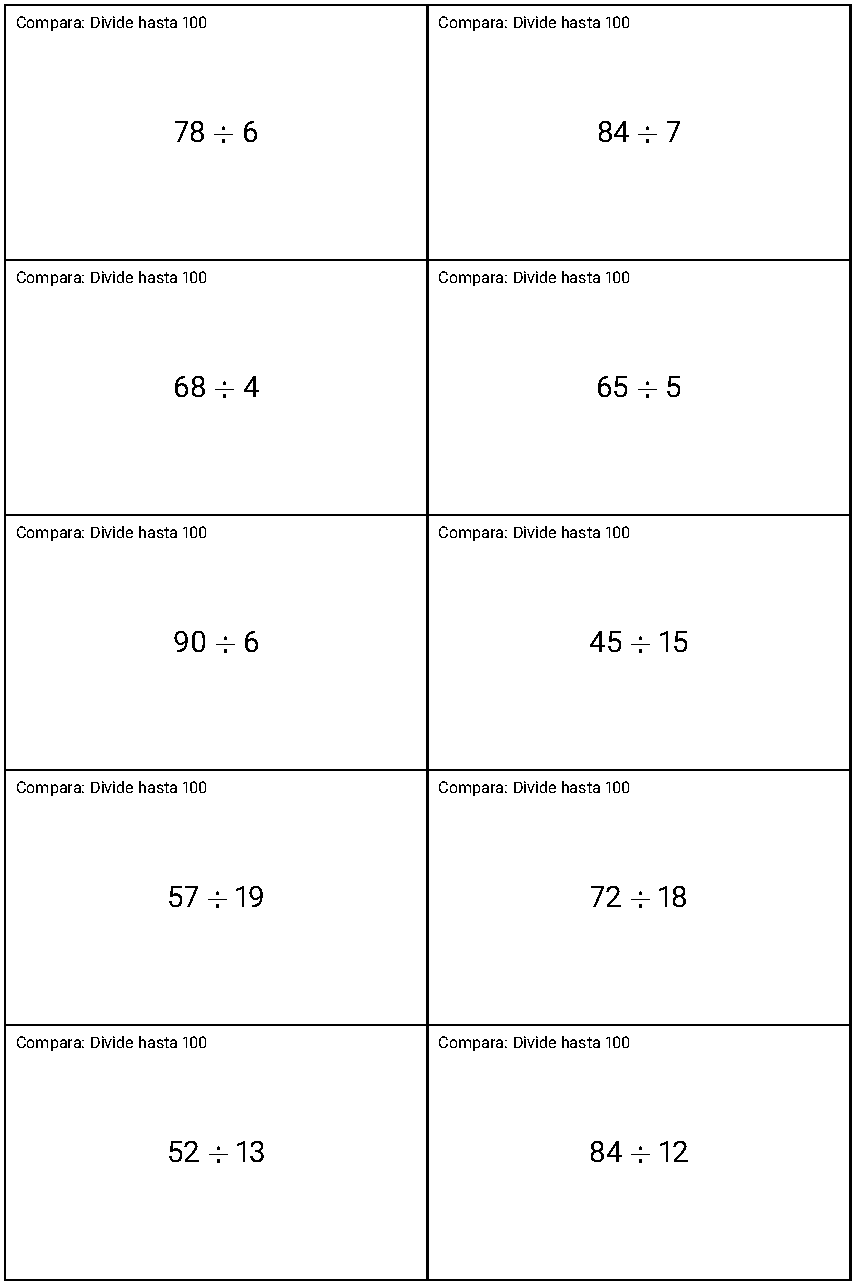
\includegraphics[max width=0.9\linewidth, center]{external/blm/tikz-source/act-comparaDivideHasta100-tarjetas-grandes1.pdf}
% \end{image}%
\cleardoublepage
% \begin{image}{0}{1}{0}{}%
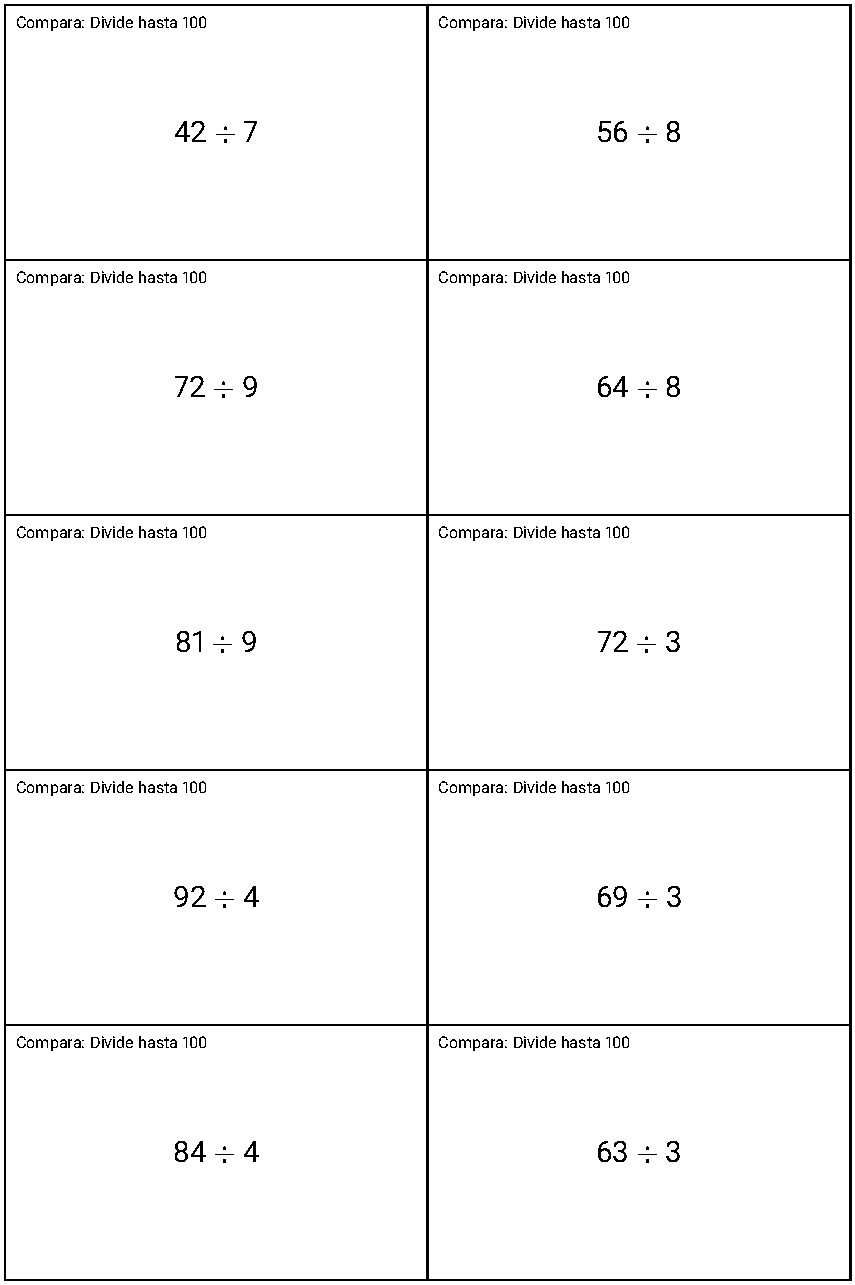
\includegraphics[max width=0.9\linewidth, center]{external/blm/tikz-source/act-comparaDivideHasta100-tarjetas-grandes2.pdf}
% \end{image}%
\cleardoublepage
\end{subsubsectionptx}
%
%
\typeout{************************************************}
\typeout{Preguntas de comprensión  Actividad de cierre}
\typeout{************************************************}
%
\begin{reading-questions-subsubsection}{Preguntas de comprensión}{Actividad de cierre}{}{Actividad de cierre}{}{}{lec-estrategiasDividir-cool}
%
\end{reading-questions-subsubsection}
\end{subsectionptx}
%
%
\typeout{************************************************}
\typeout{Subsección  Lección 21 -~Resolvamos problemas usando las cuatro operaciones}
\typeout{************************************************}
%
\begin{subsectionptx}{Subsección}{Lección 21 -~Resolvamos problemas usando las cuatro operaciones}{}{Lección 21}{}{}{lec-problemas4Operaciones}
%
%
\typeout{************************************************}
\typeout{Subsubsección  Actividad 1}
\typeout{************************************************}
%
\begin{subsubsectionptx}{Subsubsección}{Actividad 1}{}{Actividad 1}{}{}{lec-problemas4Operaciones-act1}
\begin{activity}{Actividad}{Una aventura con manzanas.}{act-unaAventuraConManzanas}%
\begin{sidebyside}{2}{0}{0}{0.1}%
\begin{sbspanel}{0.6}%
Un agricultor recogió algunas manzanas. Algunas de las manzanas están empacadas en cajas y algunas no.%
\end{sbspanel}%
\begin{sbspanel}{0.3}%
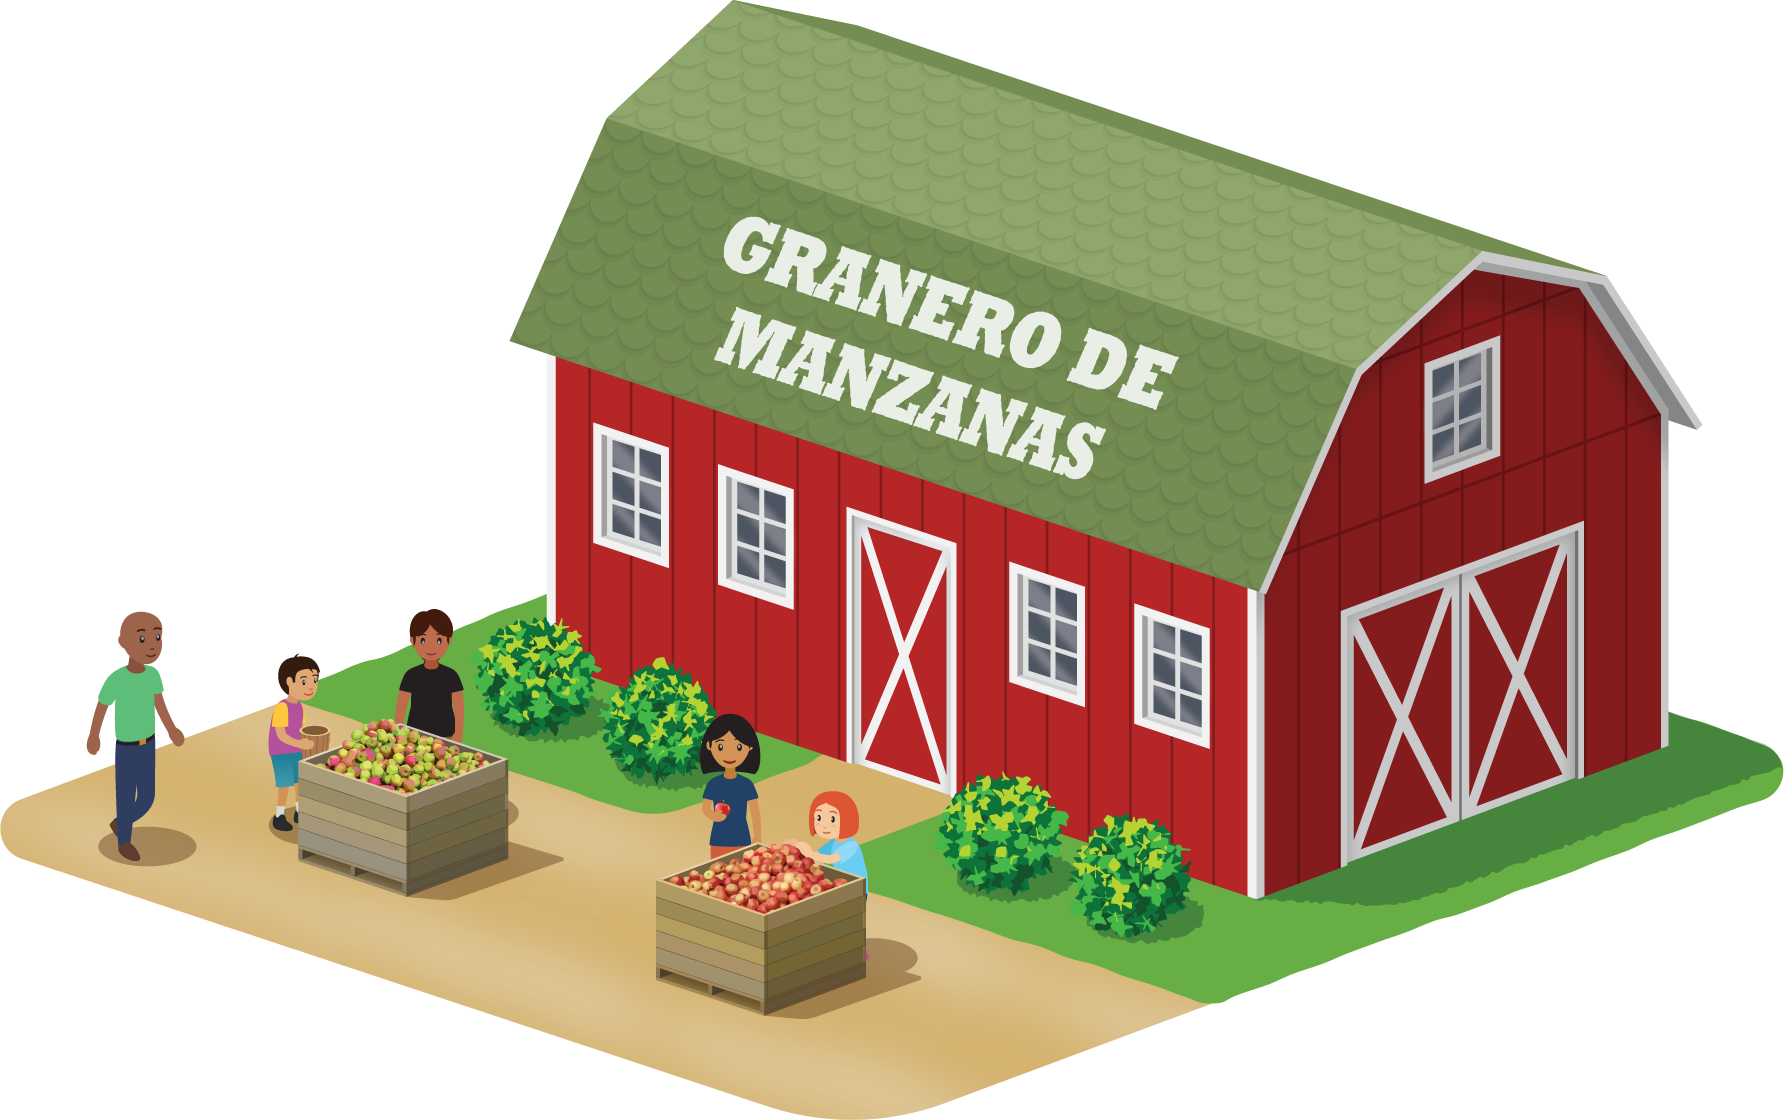
\includegraphics[max width=\linewidth, center]{external/png-source/3.4.D21.S_Sp.png}
\end{sbspanel}%
\end{sidebyside}%
\par
Escoge \(4\) números de la lista que describan correctamente la situación. Úsalos para llenar una fila de la tabla. Prepárate para explicar por qué tiene sentido juntar esos \(4\) números.%
\begin{image}{0}{1}{0}{}%
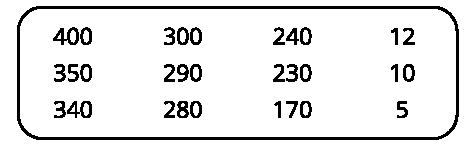
\includegraphics[max width=\linewidth, center]{external/svg-source/tikz-file-149345-scale13.pdf}
\end{image}%
\begin{image}{0}{1}{0}{}%
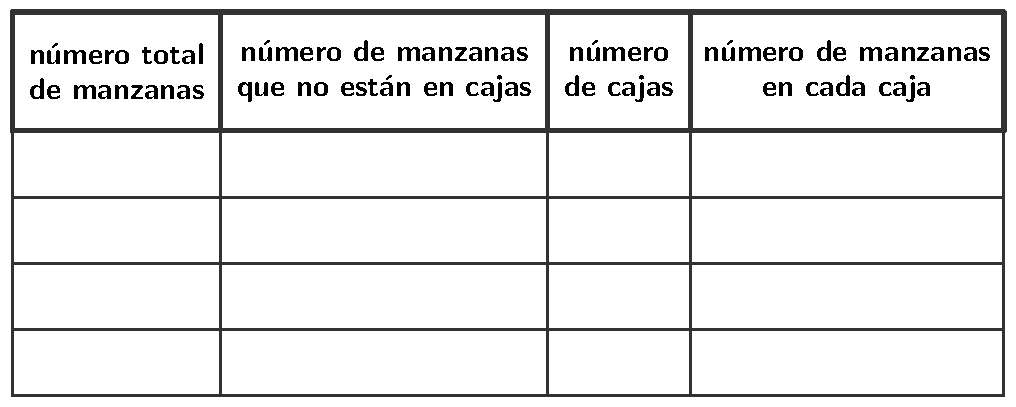
\includegraphics[max width=\linewidth, center]{external/tikz-source/3-4-21-act1-BLM-table.pdf}
\end{image}%
\end{activity}%
\end{subsubsectionptx}
%
%
\typeout{************************************************}
\typeout{Preguntas de comprensión  Actividad de cierre}
\typeout{************************************************}
%
\begin{reading-questions-subsubsection}{Preguntas de comprensión}{Actividad de cierre}{}{Actividad de cierre}{}{}{lec-problemas4Operaciones-cool}
%
\end{reading-questions-subsubsection}
\end{subsectionptx}
%
%
\typeout{************************************************}
\typeout{Subsección  Lección 22 -~La huerta comunitaria de la escuela}
\typeout{************************************************}
%
\begin{subsectionptx}{Subsección}{Lección 22 -~La huerta comunitaria de la escuela}{}{Lección 22}{}{}{lec-huertaComunitaria}
\end{subsectionptx}
%
%
\typeout{************************************************}
\typeout{Ejercicios  Problemas de práctica de la sección D}
\typeout{************************************************}
%
\begin{exercises-subsection}{Ejercicios}{Problemas de práctica de la sección D}{}{Problemas de práctica}{}{}{gra3-uni4-secD-ProblemasPractica}
%
% \vspace{2cm}
%
%
%
%
%
%
\end{exercises-subsection}
\end{sectionptx}
%
%
% \clearpage
\typeout{************************************************}
\typeout{Referencias  Atribuciones de imágenes}
\typeout{************************************************}
%
% \begin{references-section}{Referencias}{Atribuciones de imágenes}{}{Atribuciones de imágenes}{}{}{gra3-uni4-9}
% %
% \begin{itemize}[label=\textbullet]
% \item{}\hyperref[act-clasificacionDeTarjetas-todoSobreBichos]{Clasificación de tarjetas: Todo sobre bichos, p.\,\pageref{act-clasificacionDeTarjetas-todoSobreBichos}} Nicholas Caffarilla. CC-BY-SA 3.0. Wikipedia. \href{https://en.wikipedia.org/wiki/File:Insect_collage.png}{https:\slash{}\slash{}en.wikipedia.org}\footnote{\nolinkurl{en.wikipedia.org/wiki/File:Insect_collage.png}\label{gra3-uni4-9-2-4-3}}.%
% \end{itemize}
% Las imágenes sin atrubición las produjo LEMA \href{https://www.grupolema.org}{www.grupolema.org}\footnote{\nolinkurl{www.grupolema.org}\label{gra3-uni4-9-3-2}} específicamente para esta adaptación y se liberan con una licencia Creative Commons Attribution 4.0 International License (CC BY 4.0), o son © 2021 \href{https://curriculum.illustrativemathematics.org}{Illustrative Mathematics}\footnote{\nolinkurl{curriculum.illustrativemathematics.org}\label{gra3-uni4-9-3-4}} con una licencia Creative Commons Attribution 4.0 International License (CC BY 4.0) y se reproducen directamente de la versión en Español disponible en \href{https://im.kendallhunt.com/K5_ES/curriculum.html}{im.kendallhunt.com}\footnote{\nolinkurl{im.kendallhunt.com/K5_ES/curriculum.html}\label{gra3-uni4-9-3-6}}.%
% \end{references-section}
\end{document}
